\onecolumn

\begin{figure}

\centering
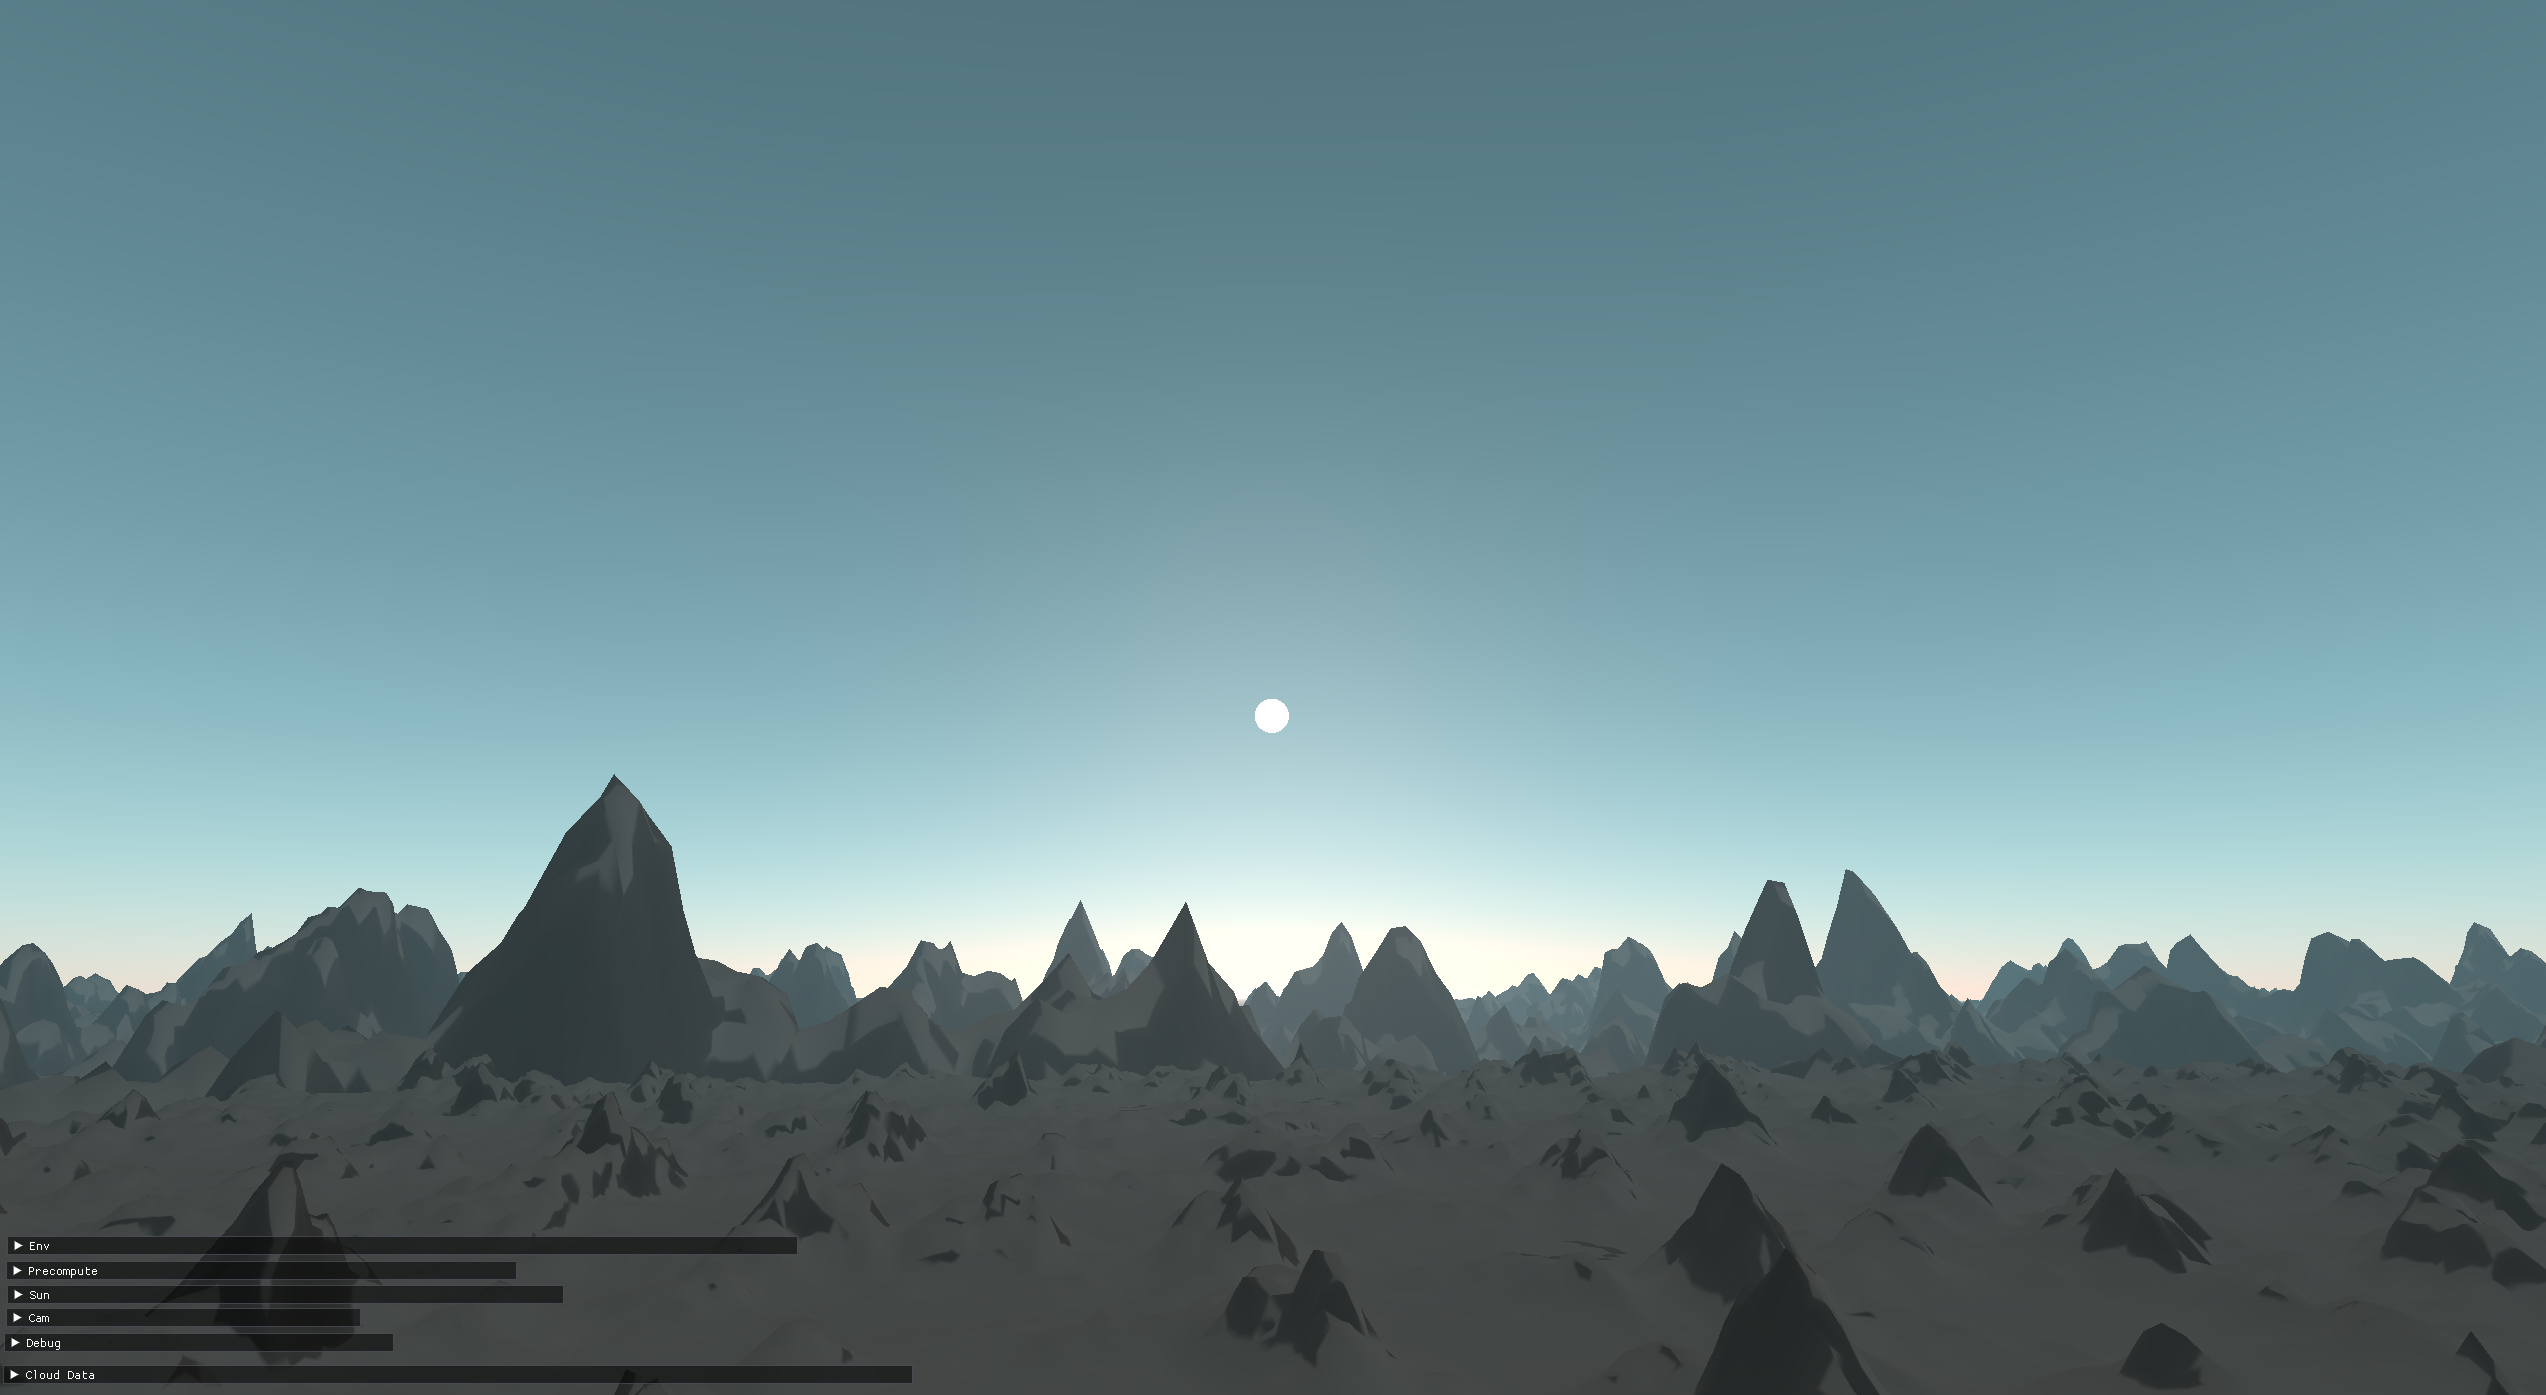
\includegraphics[scale=0.08]{noon.png} 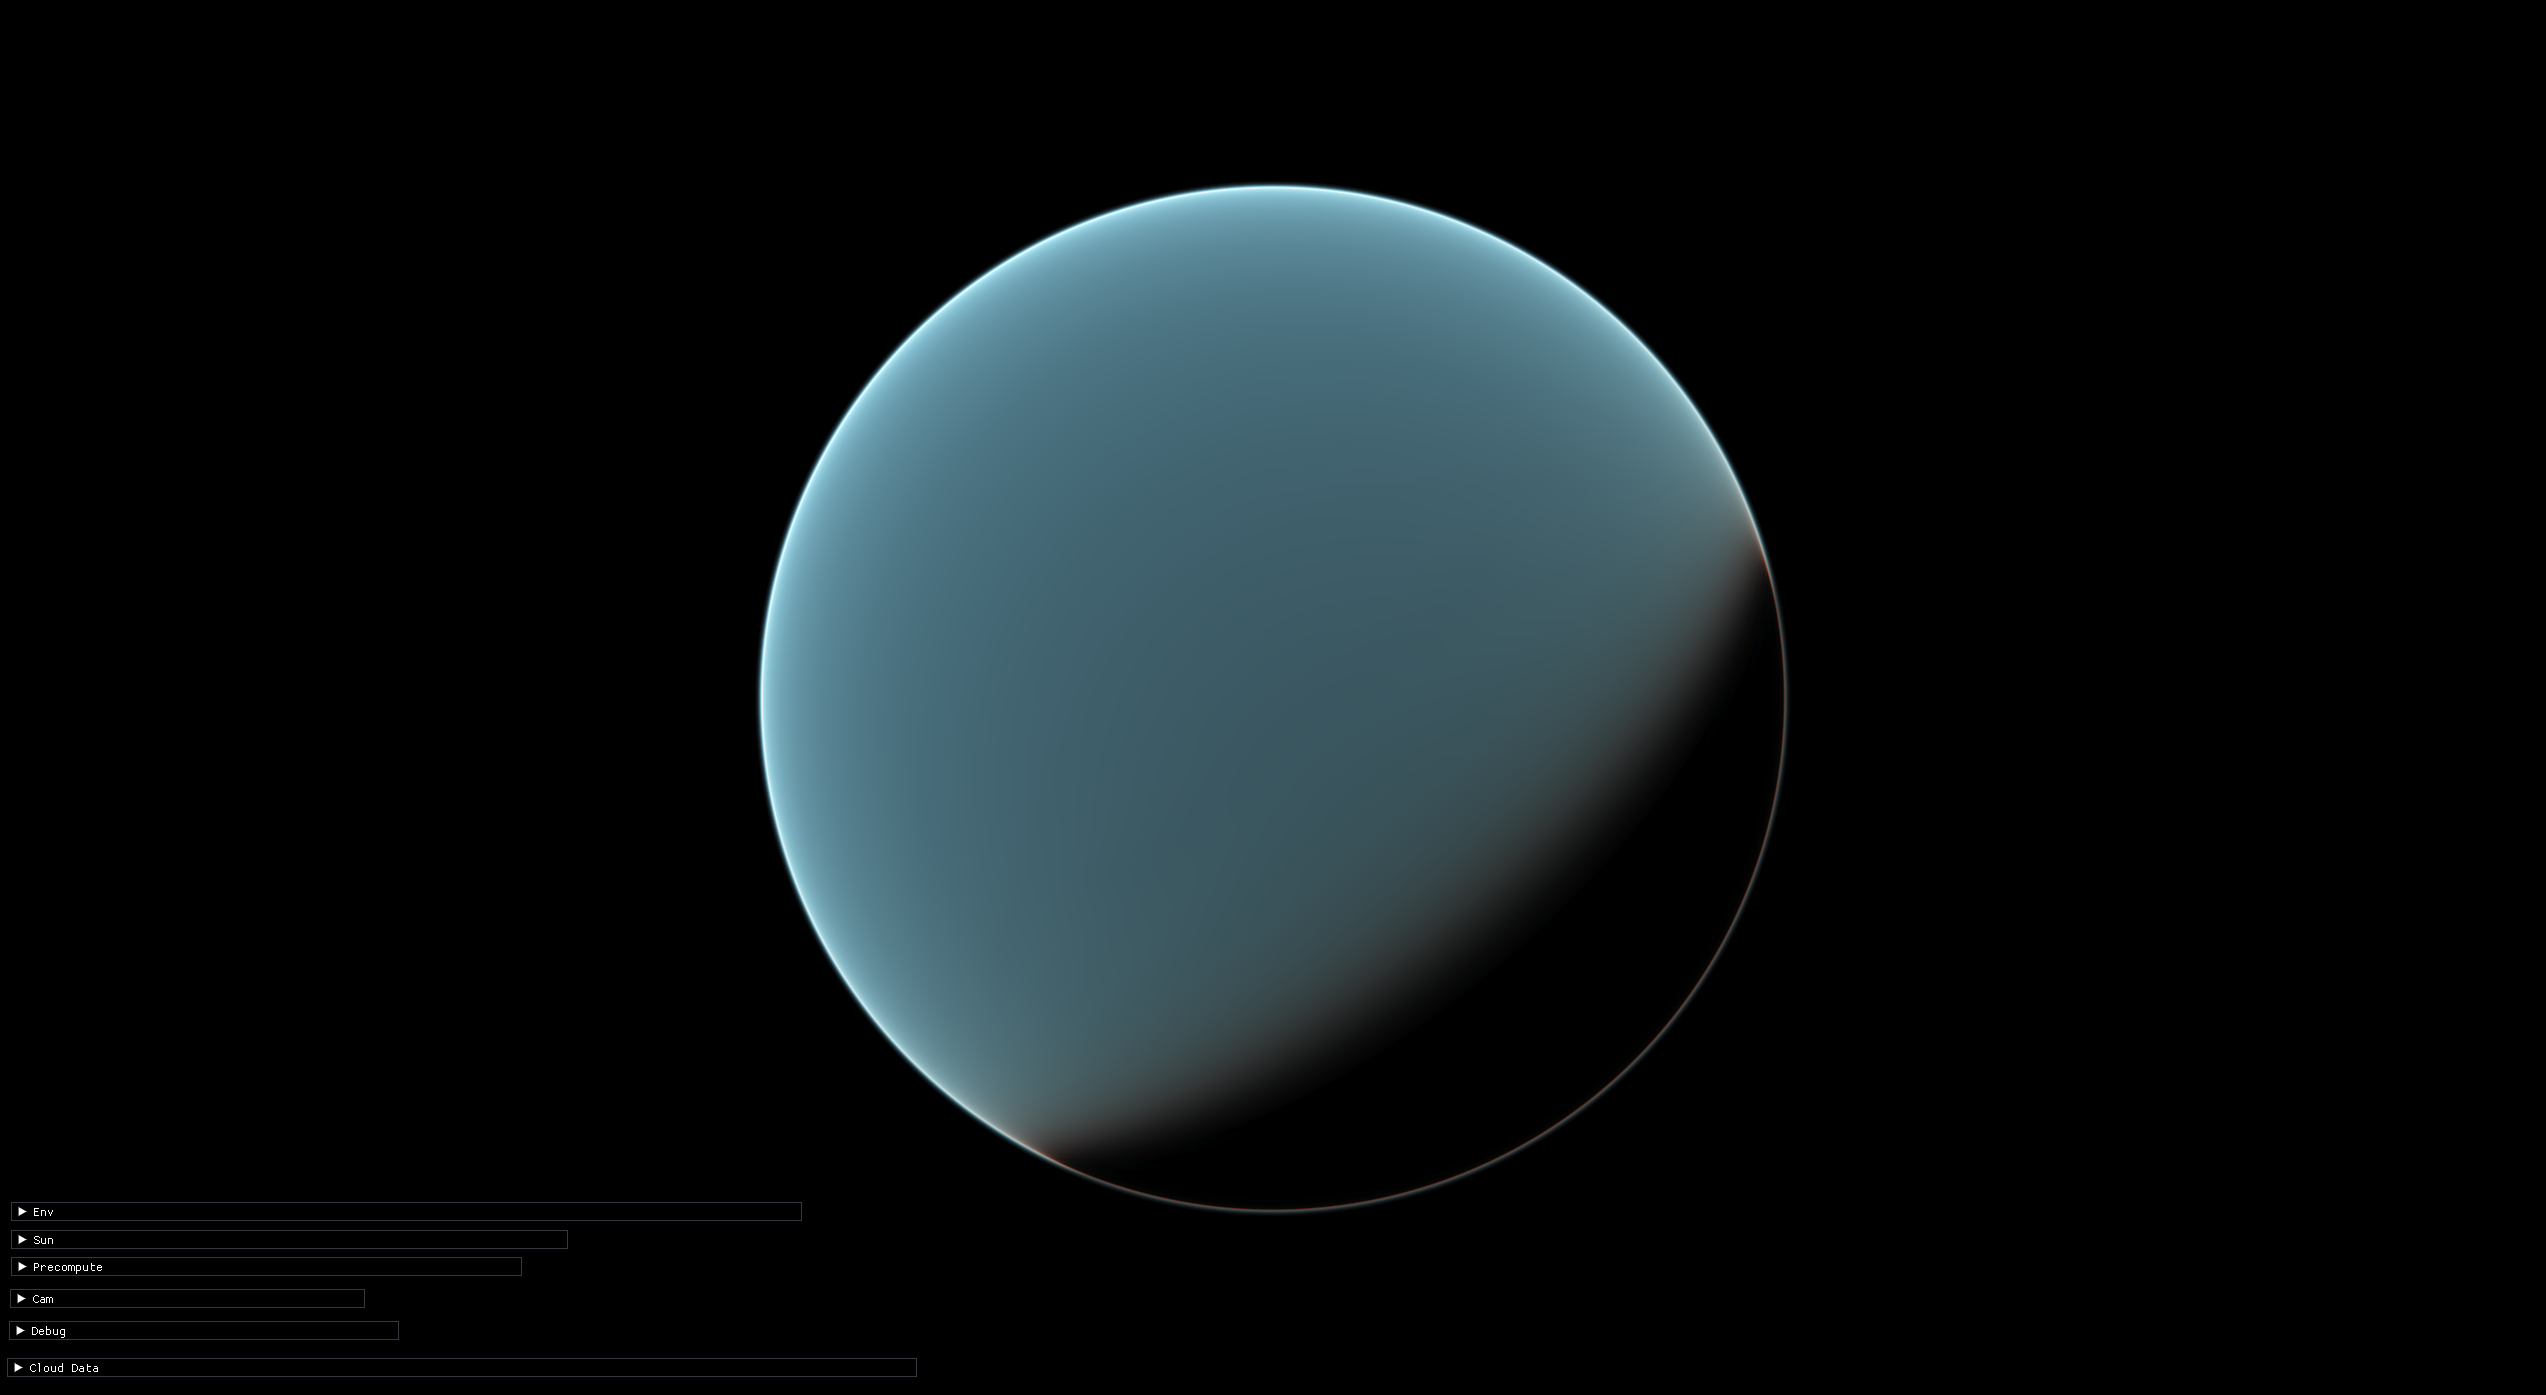
\includegraphics[scale=0.08]{space_earthlike.png}
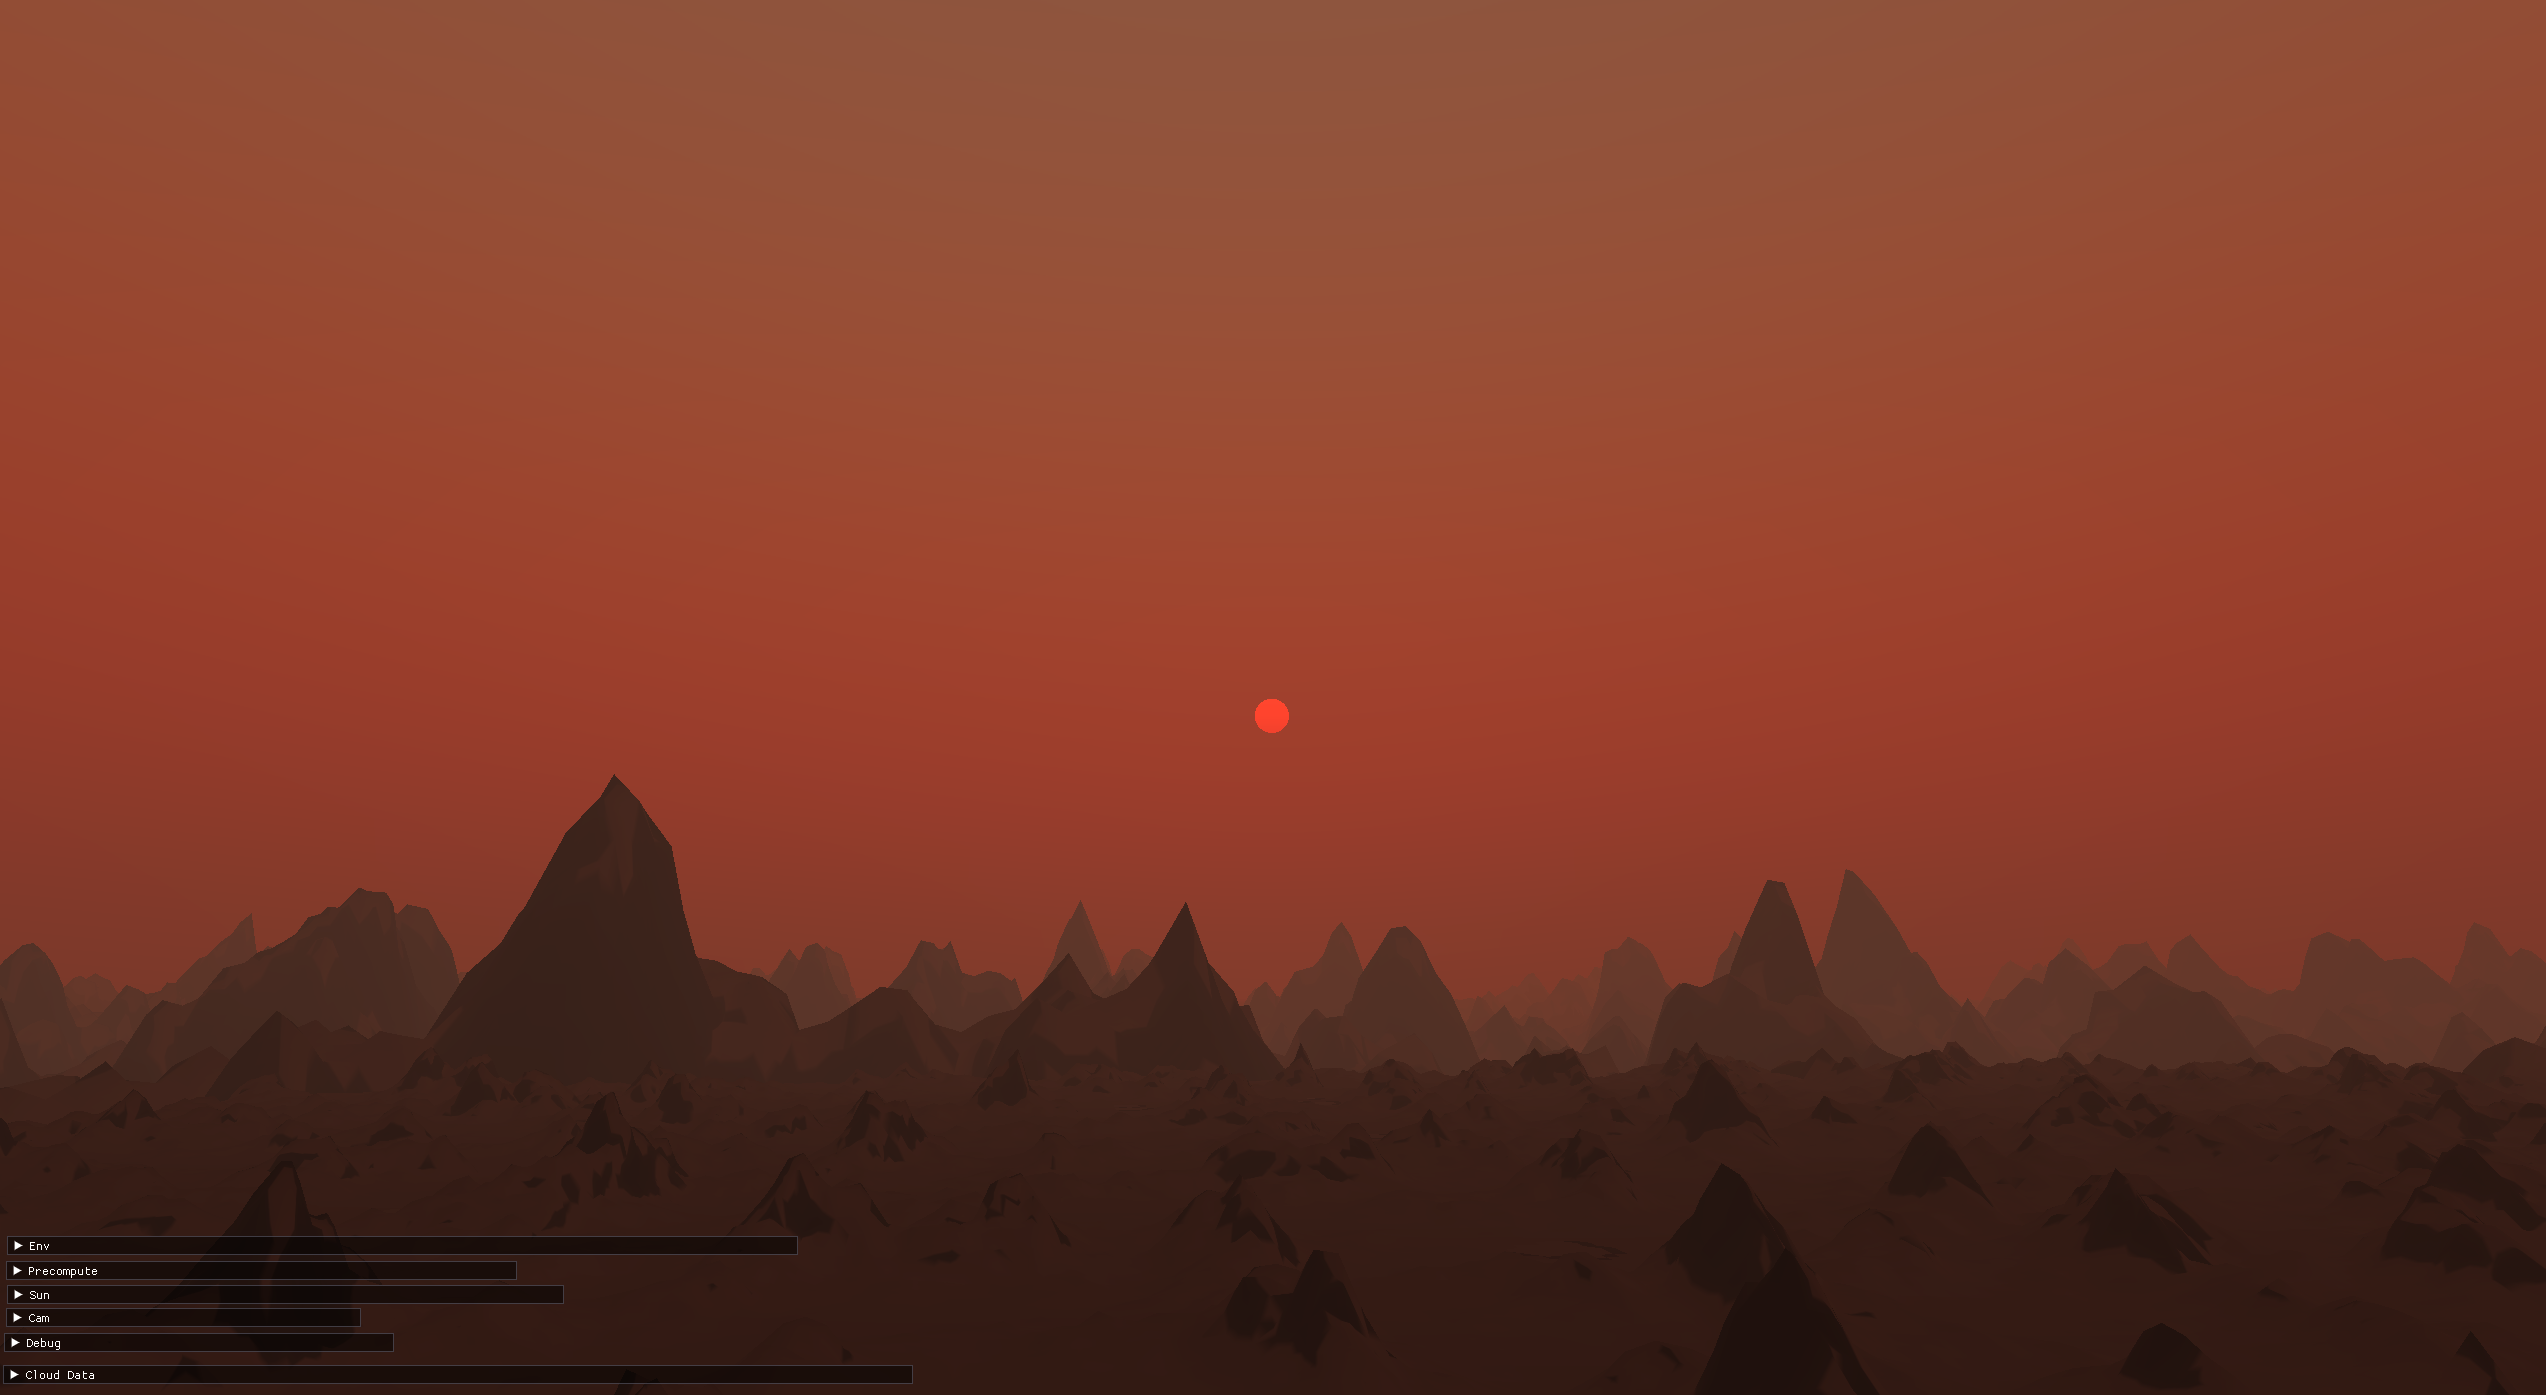
\includegraphics[scale=0.08]{dense.png} 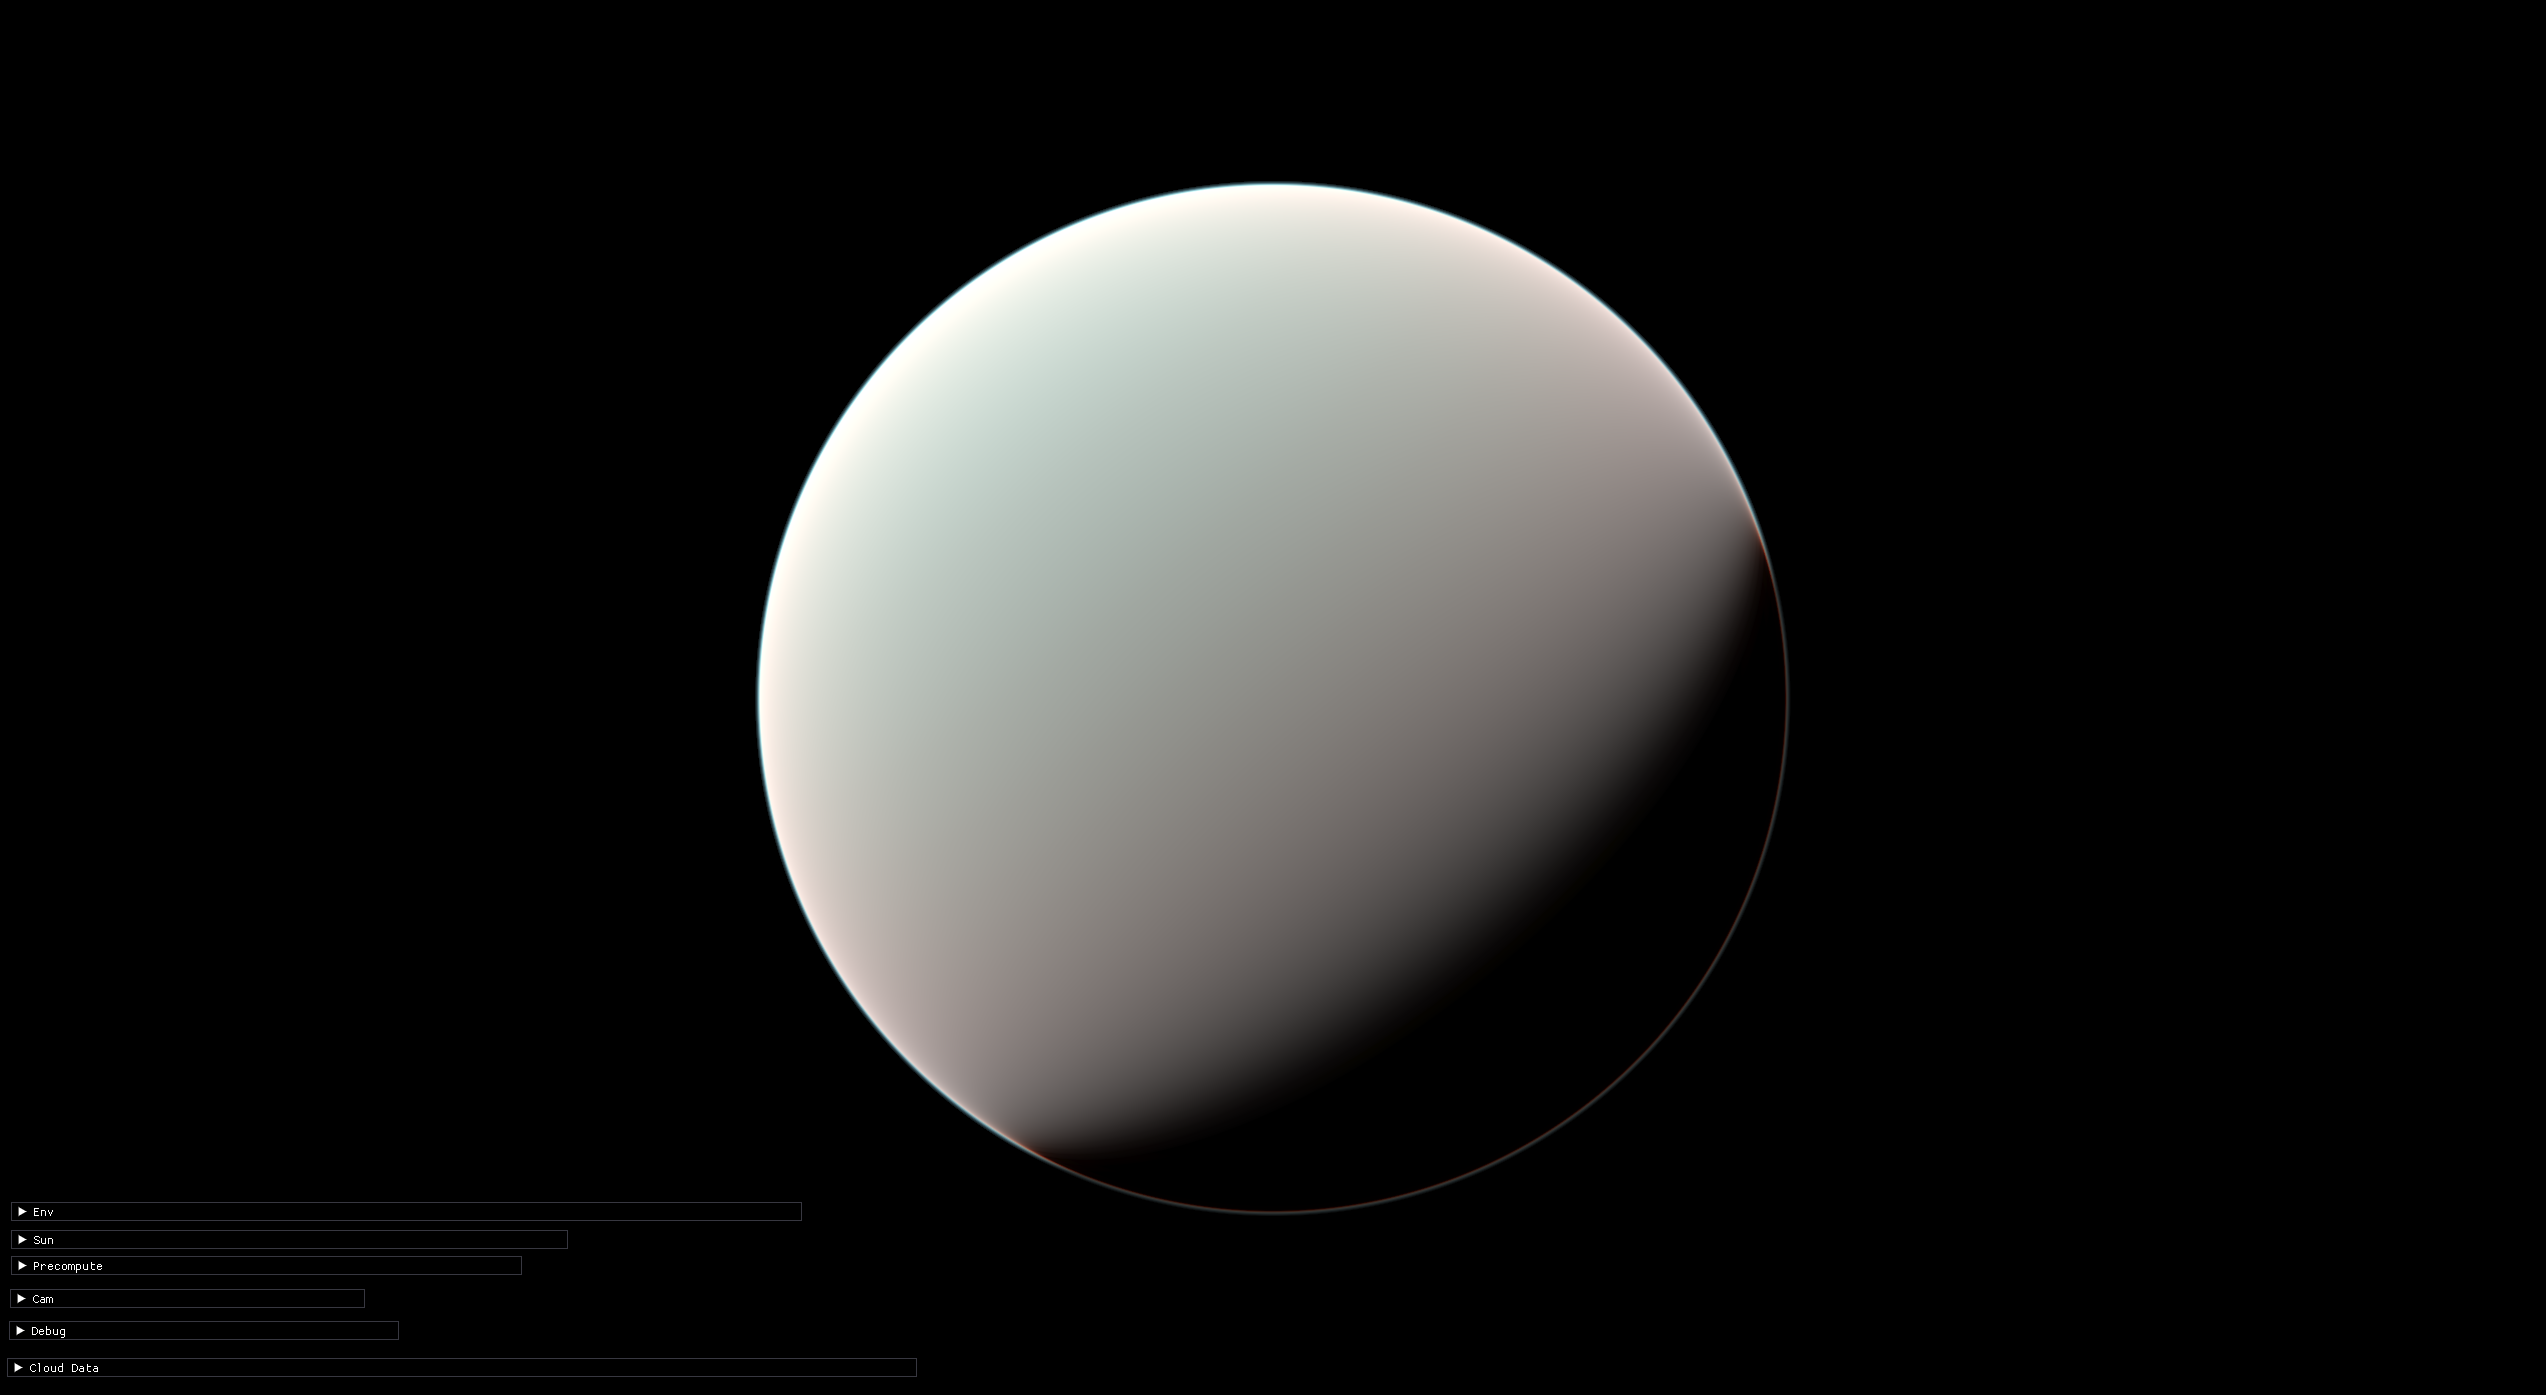
\includegraphics[scale=0.08]{space_dense.png}
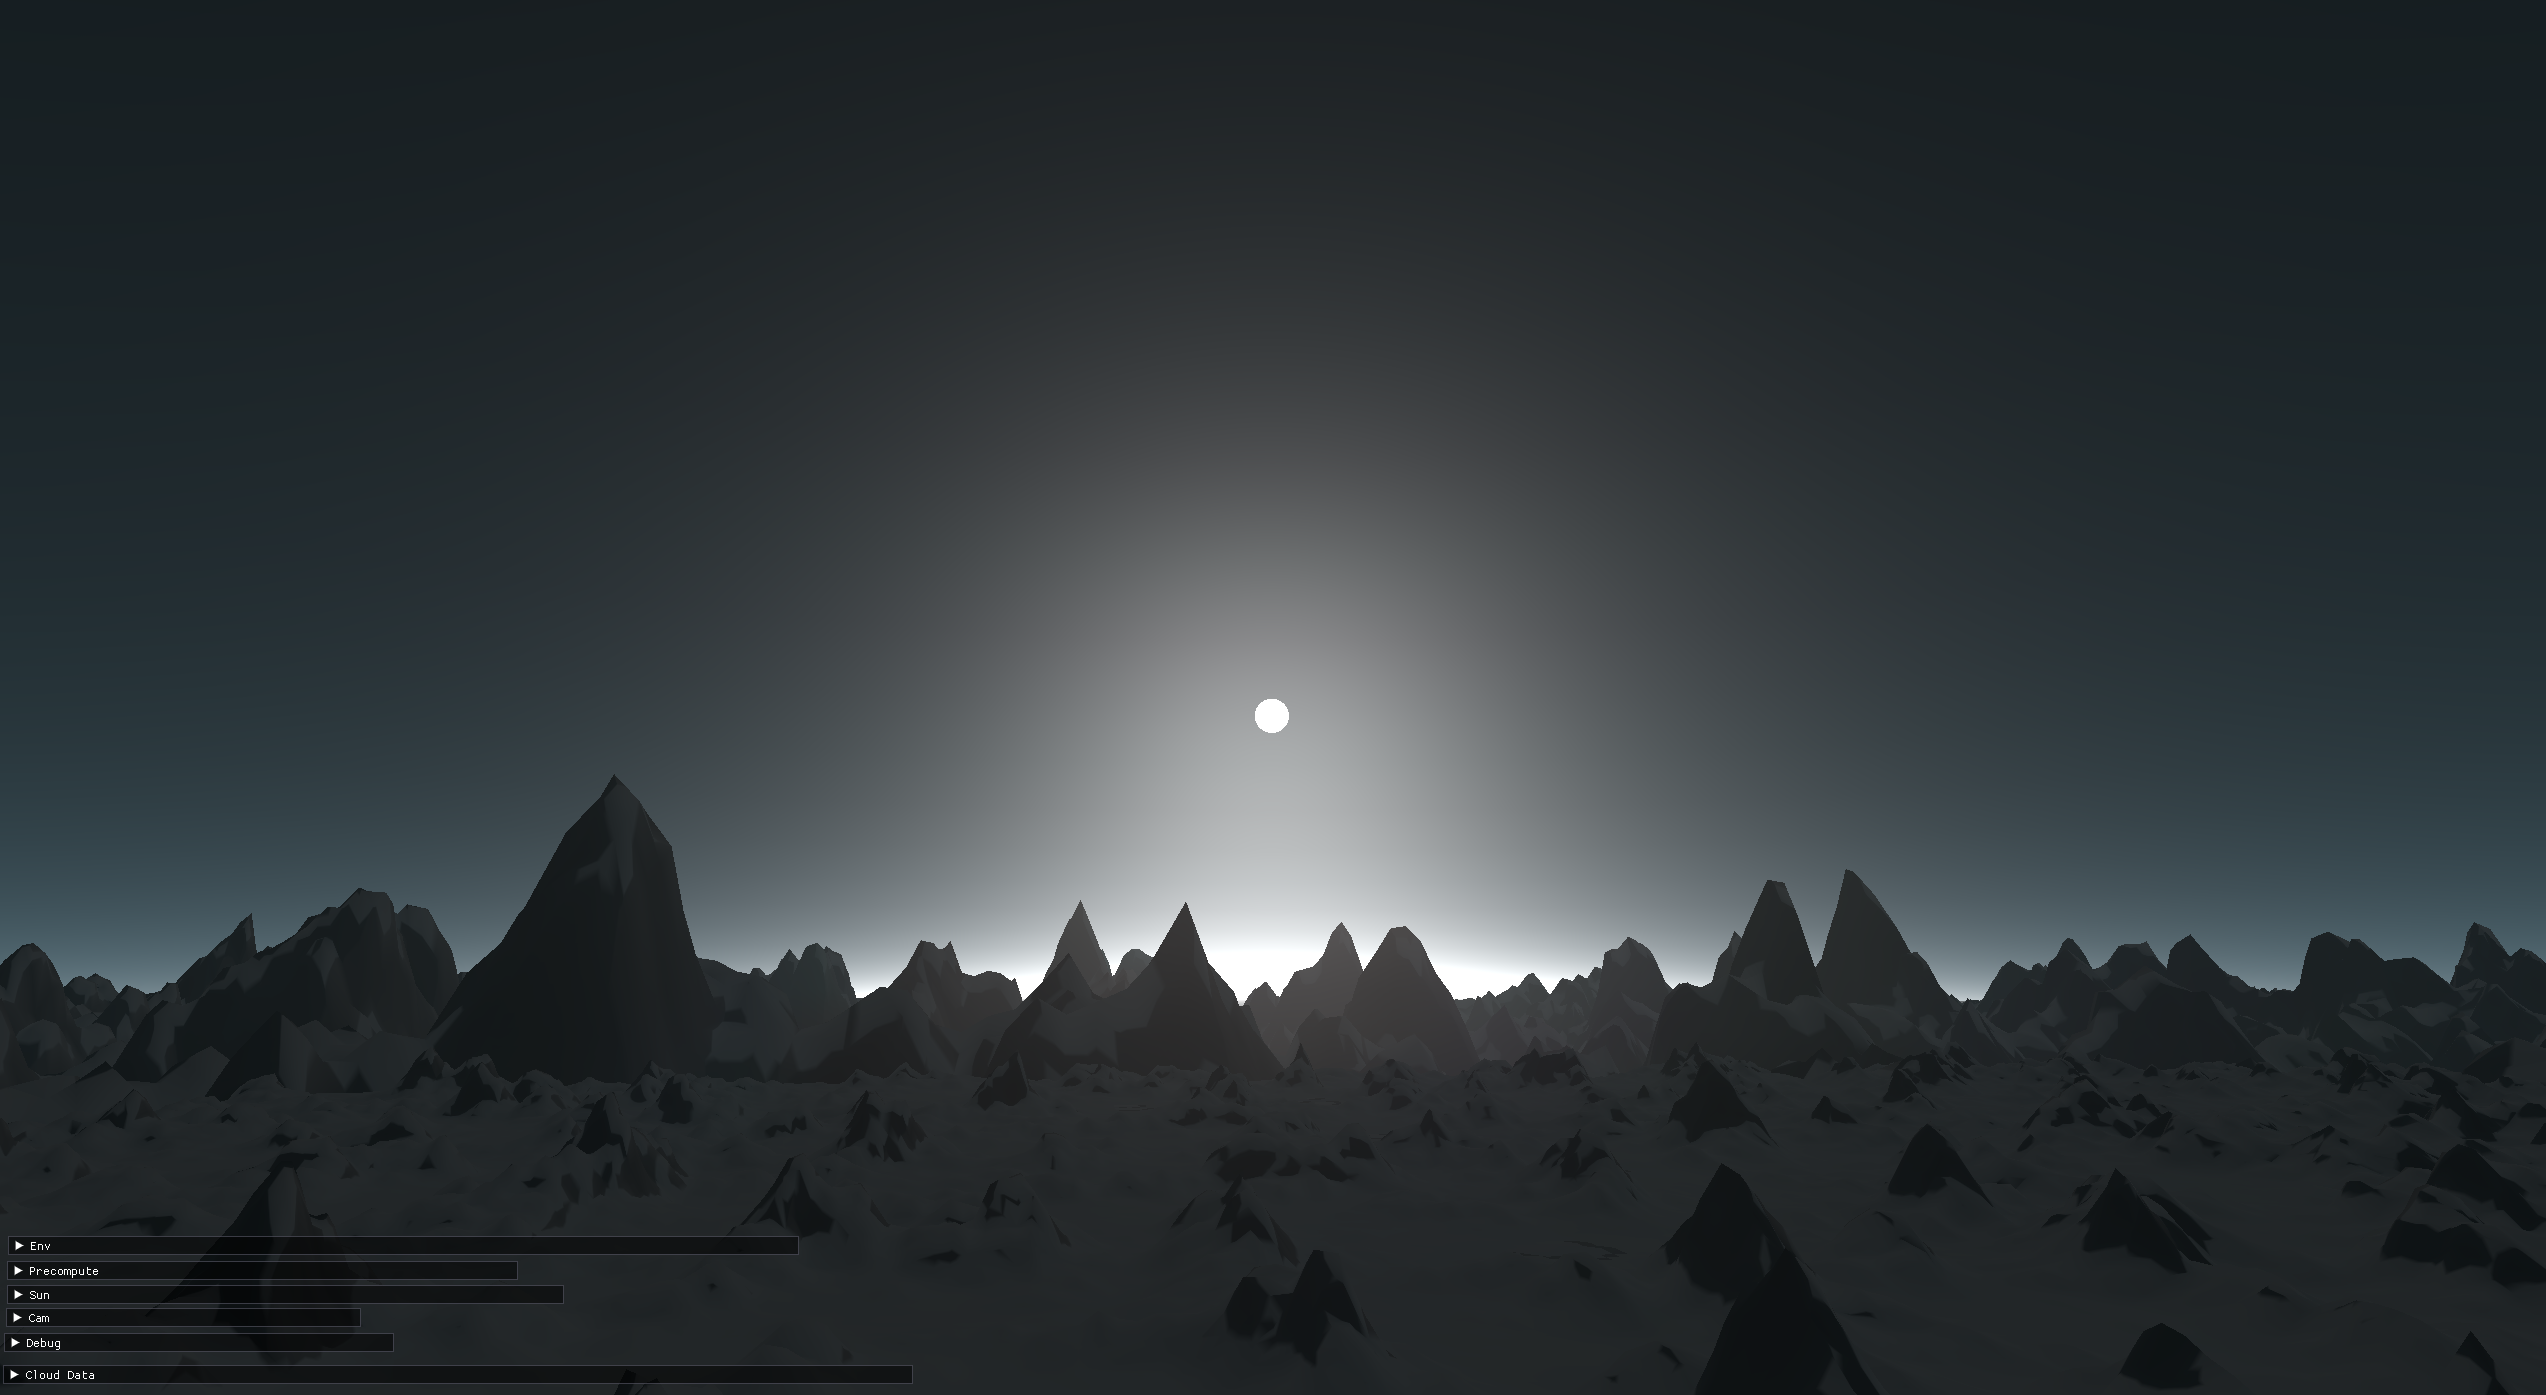
\includegraphics[scale=0.08]{low.png} 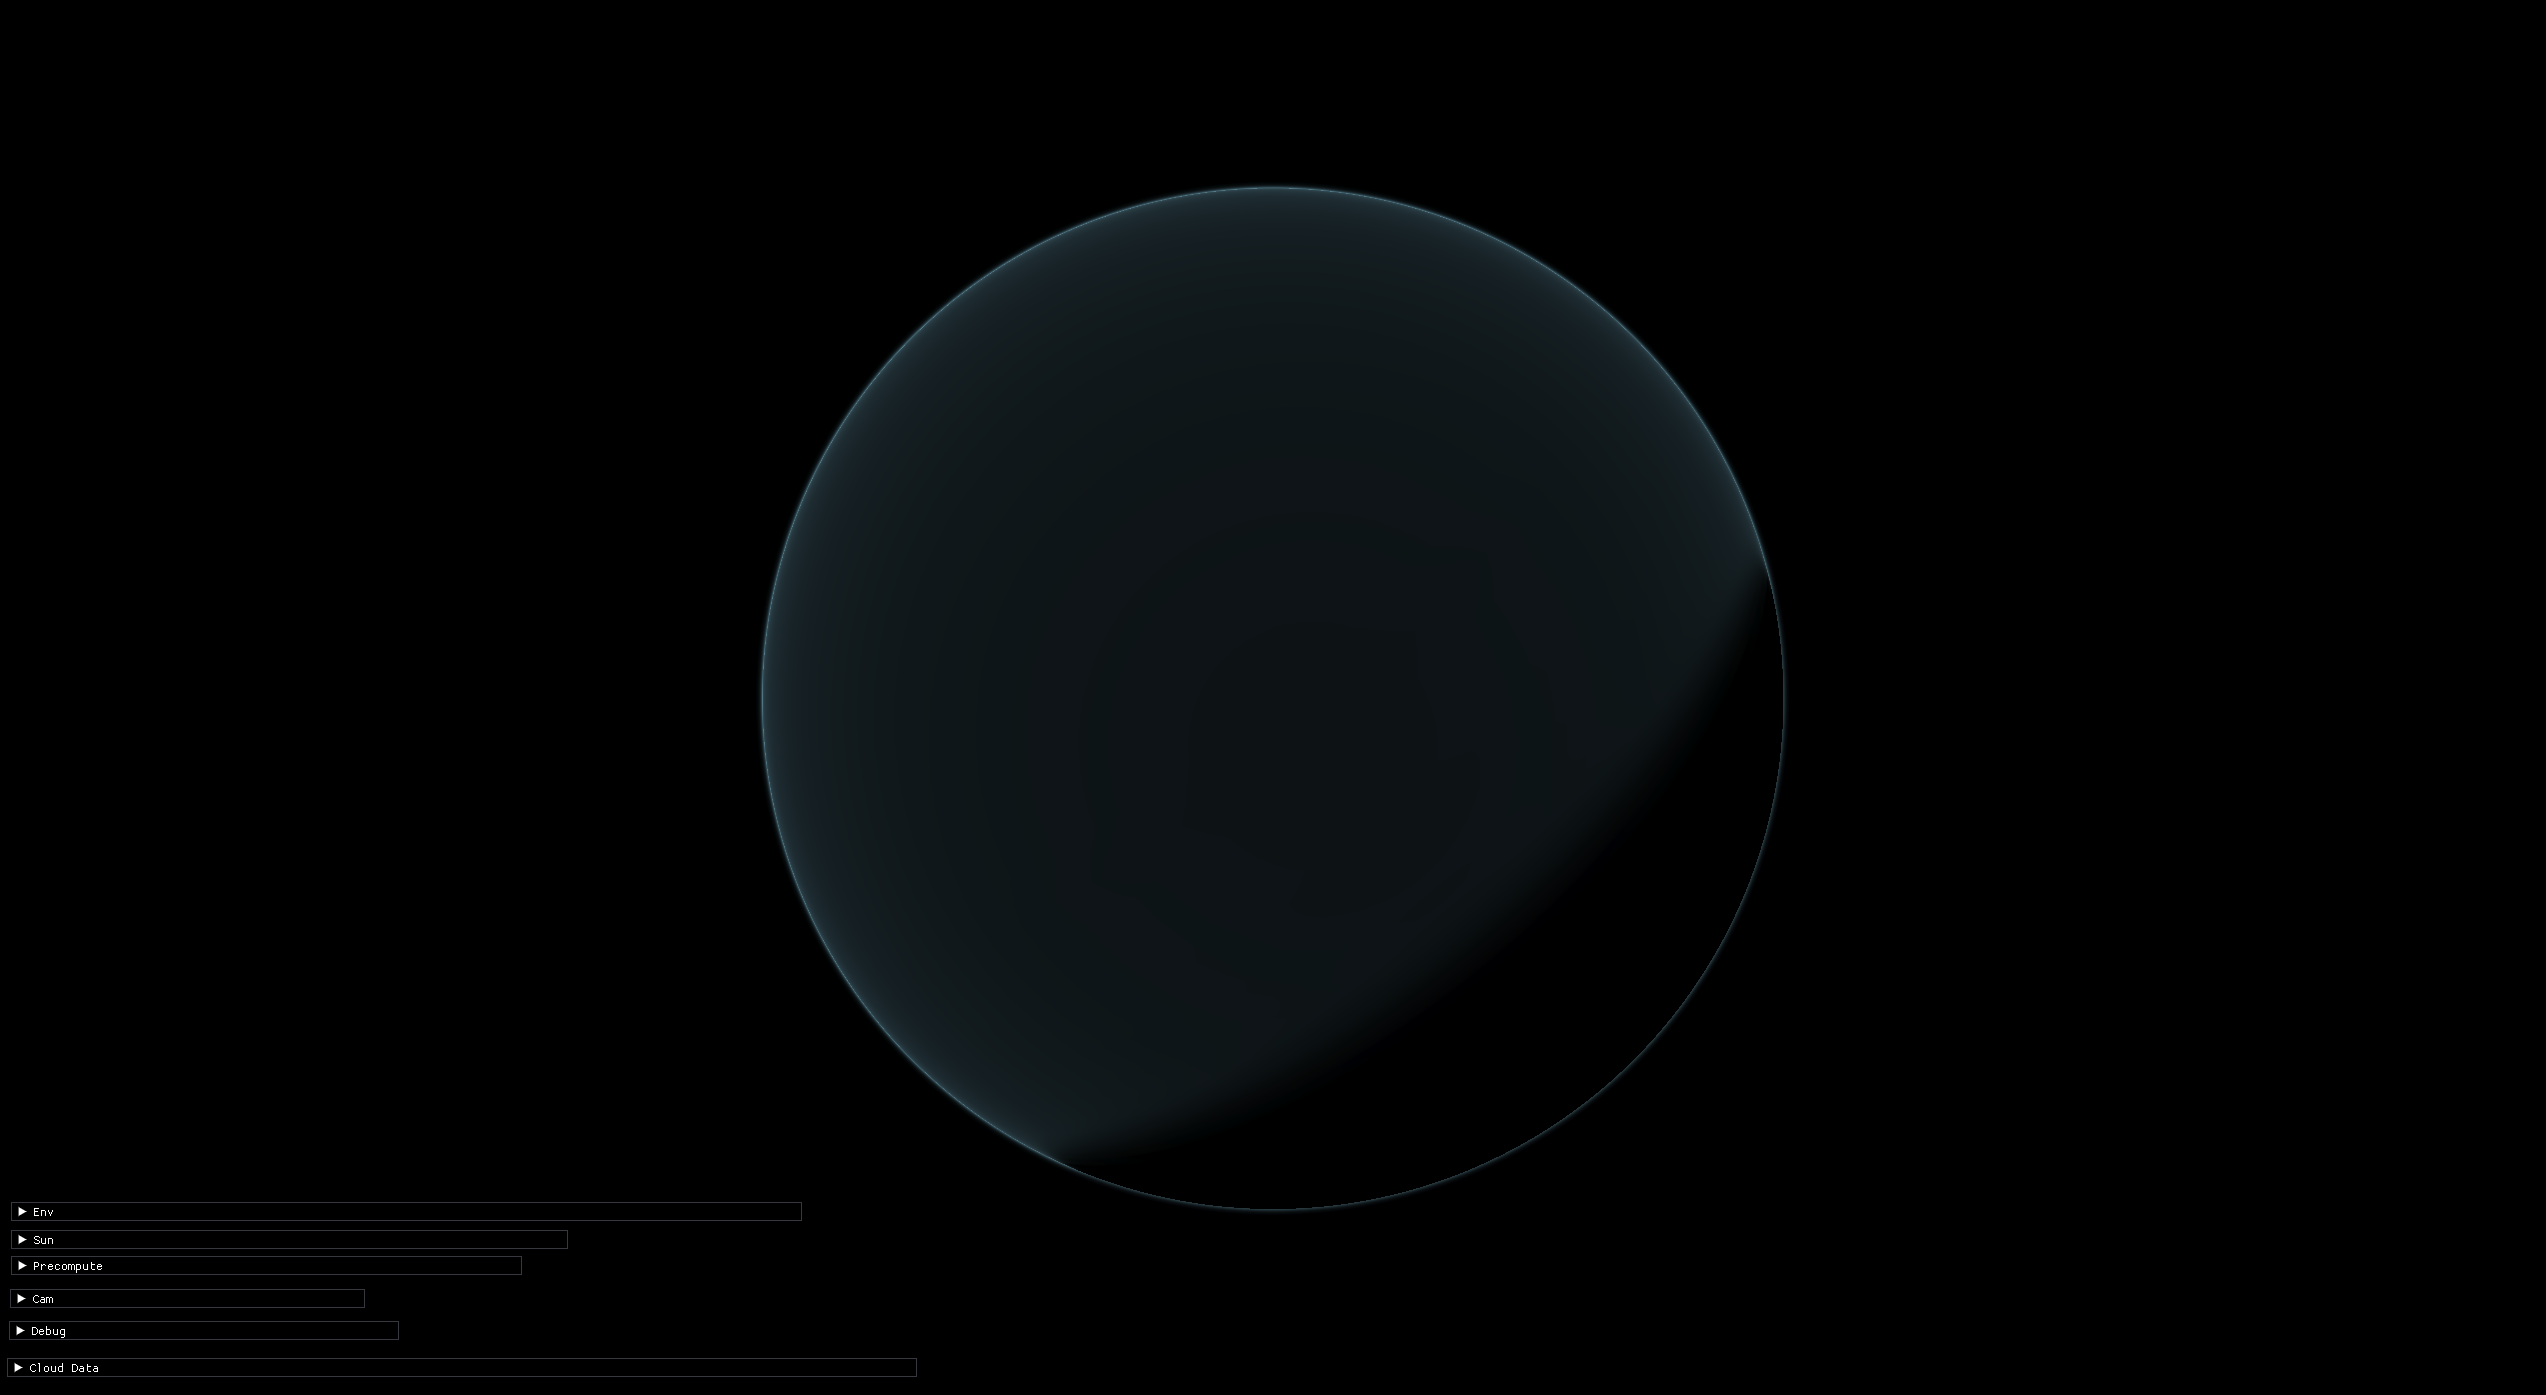
\includegraphics[scale=0.08]{space_light.png}
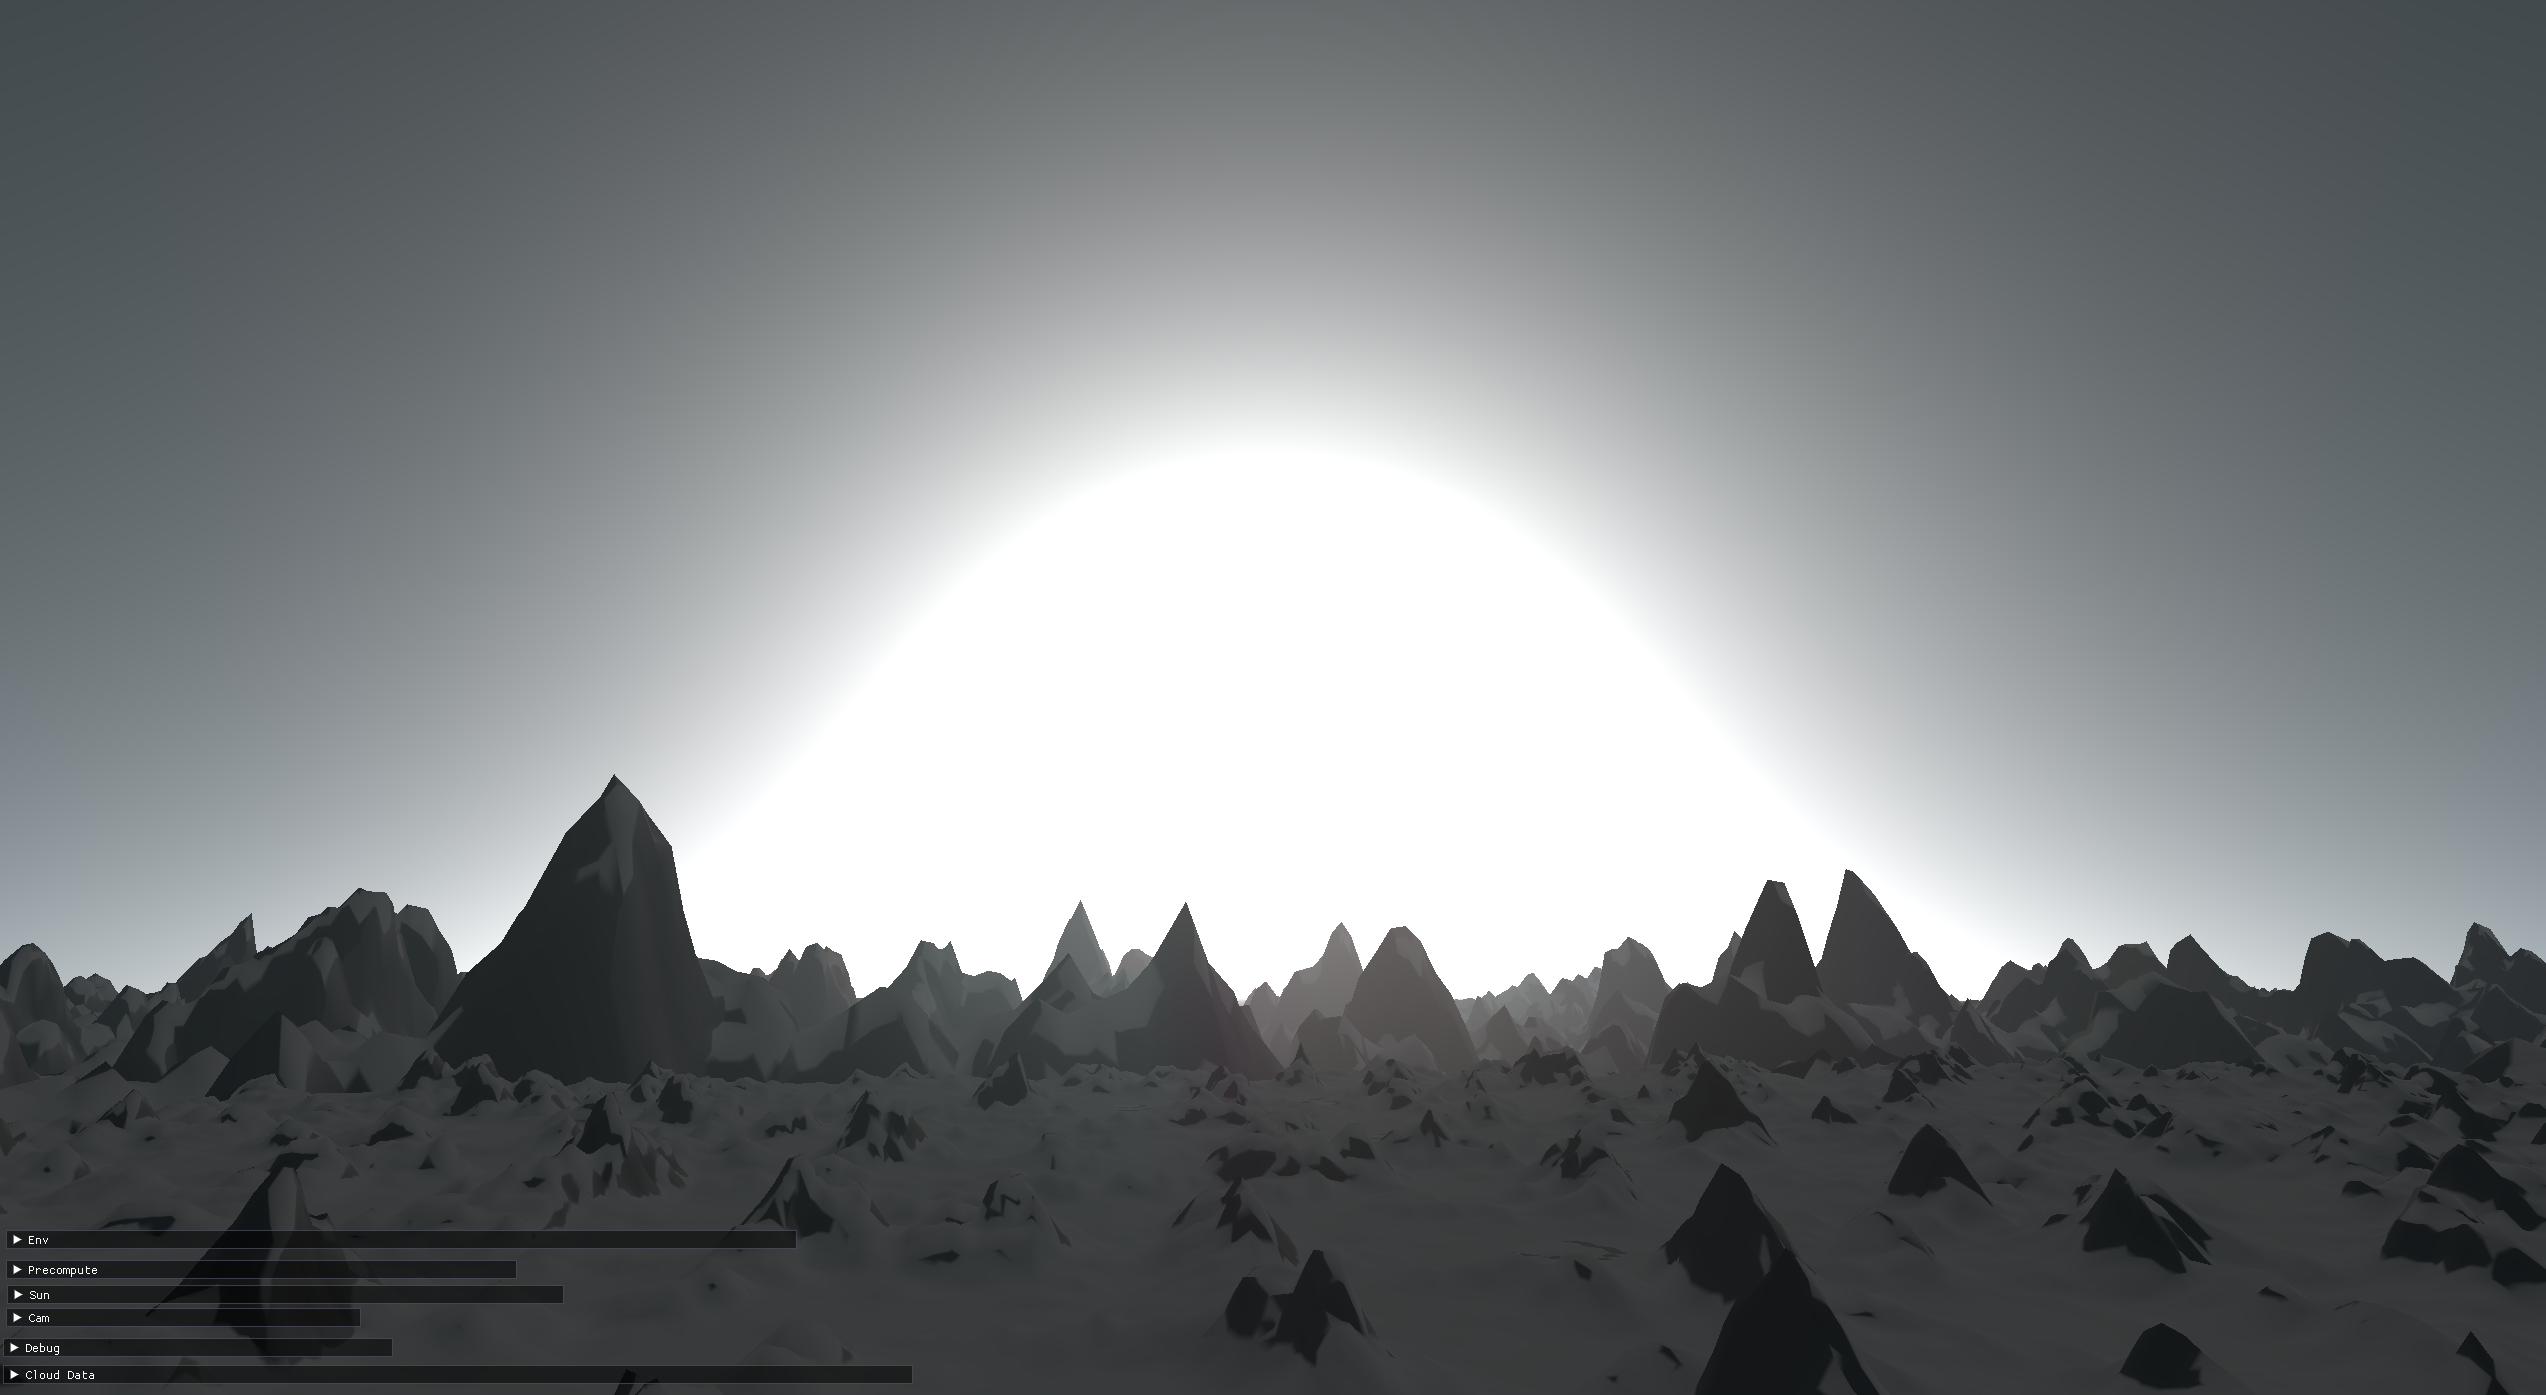
\includegraphics[scale=0.08]{big.png} 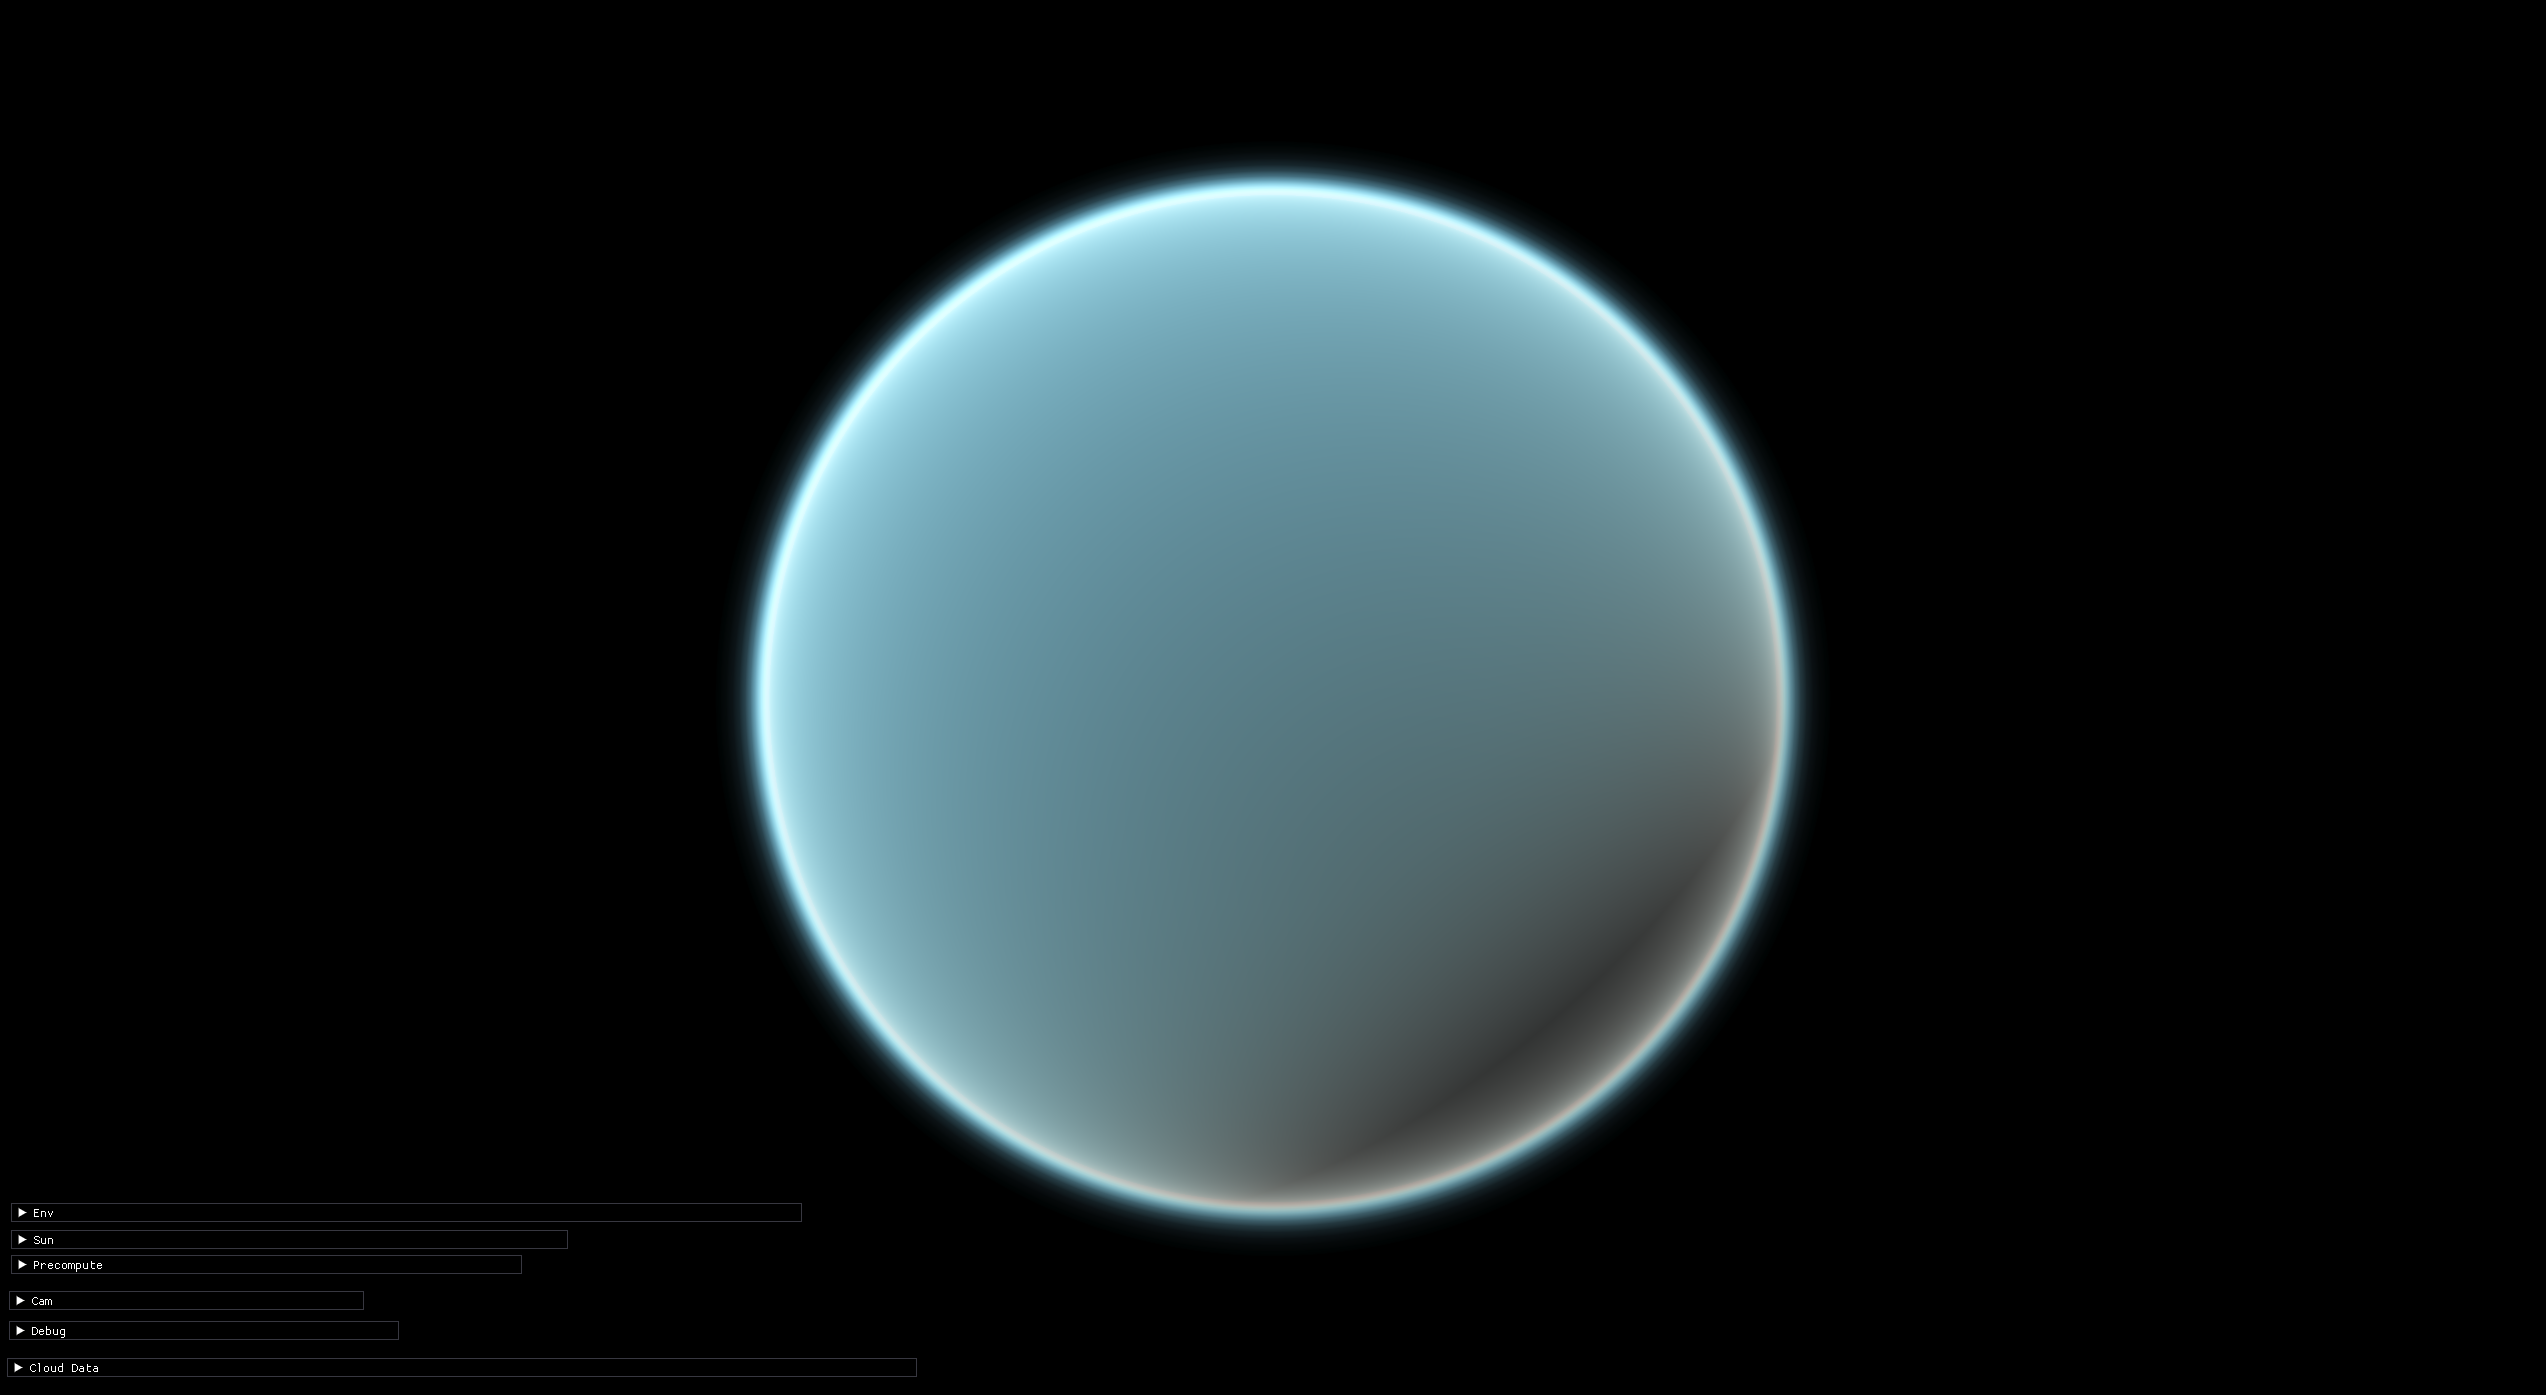
\includegraphics[scale=0.08]{space_big.png}

\centering
\caption{Erdähnliche, dichtere, dünnere und größere Atmosphäre}
\label{pics}
\end{figure}

\begin{figure}
\centering
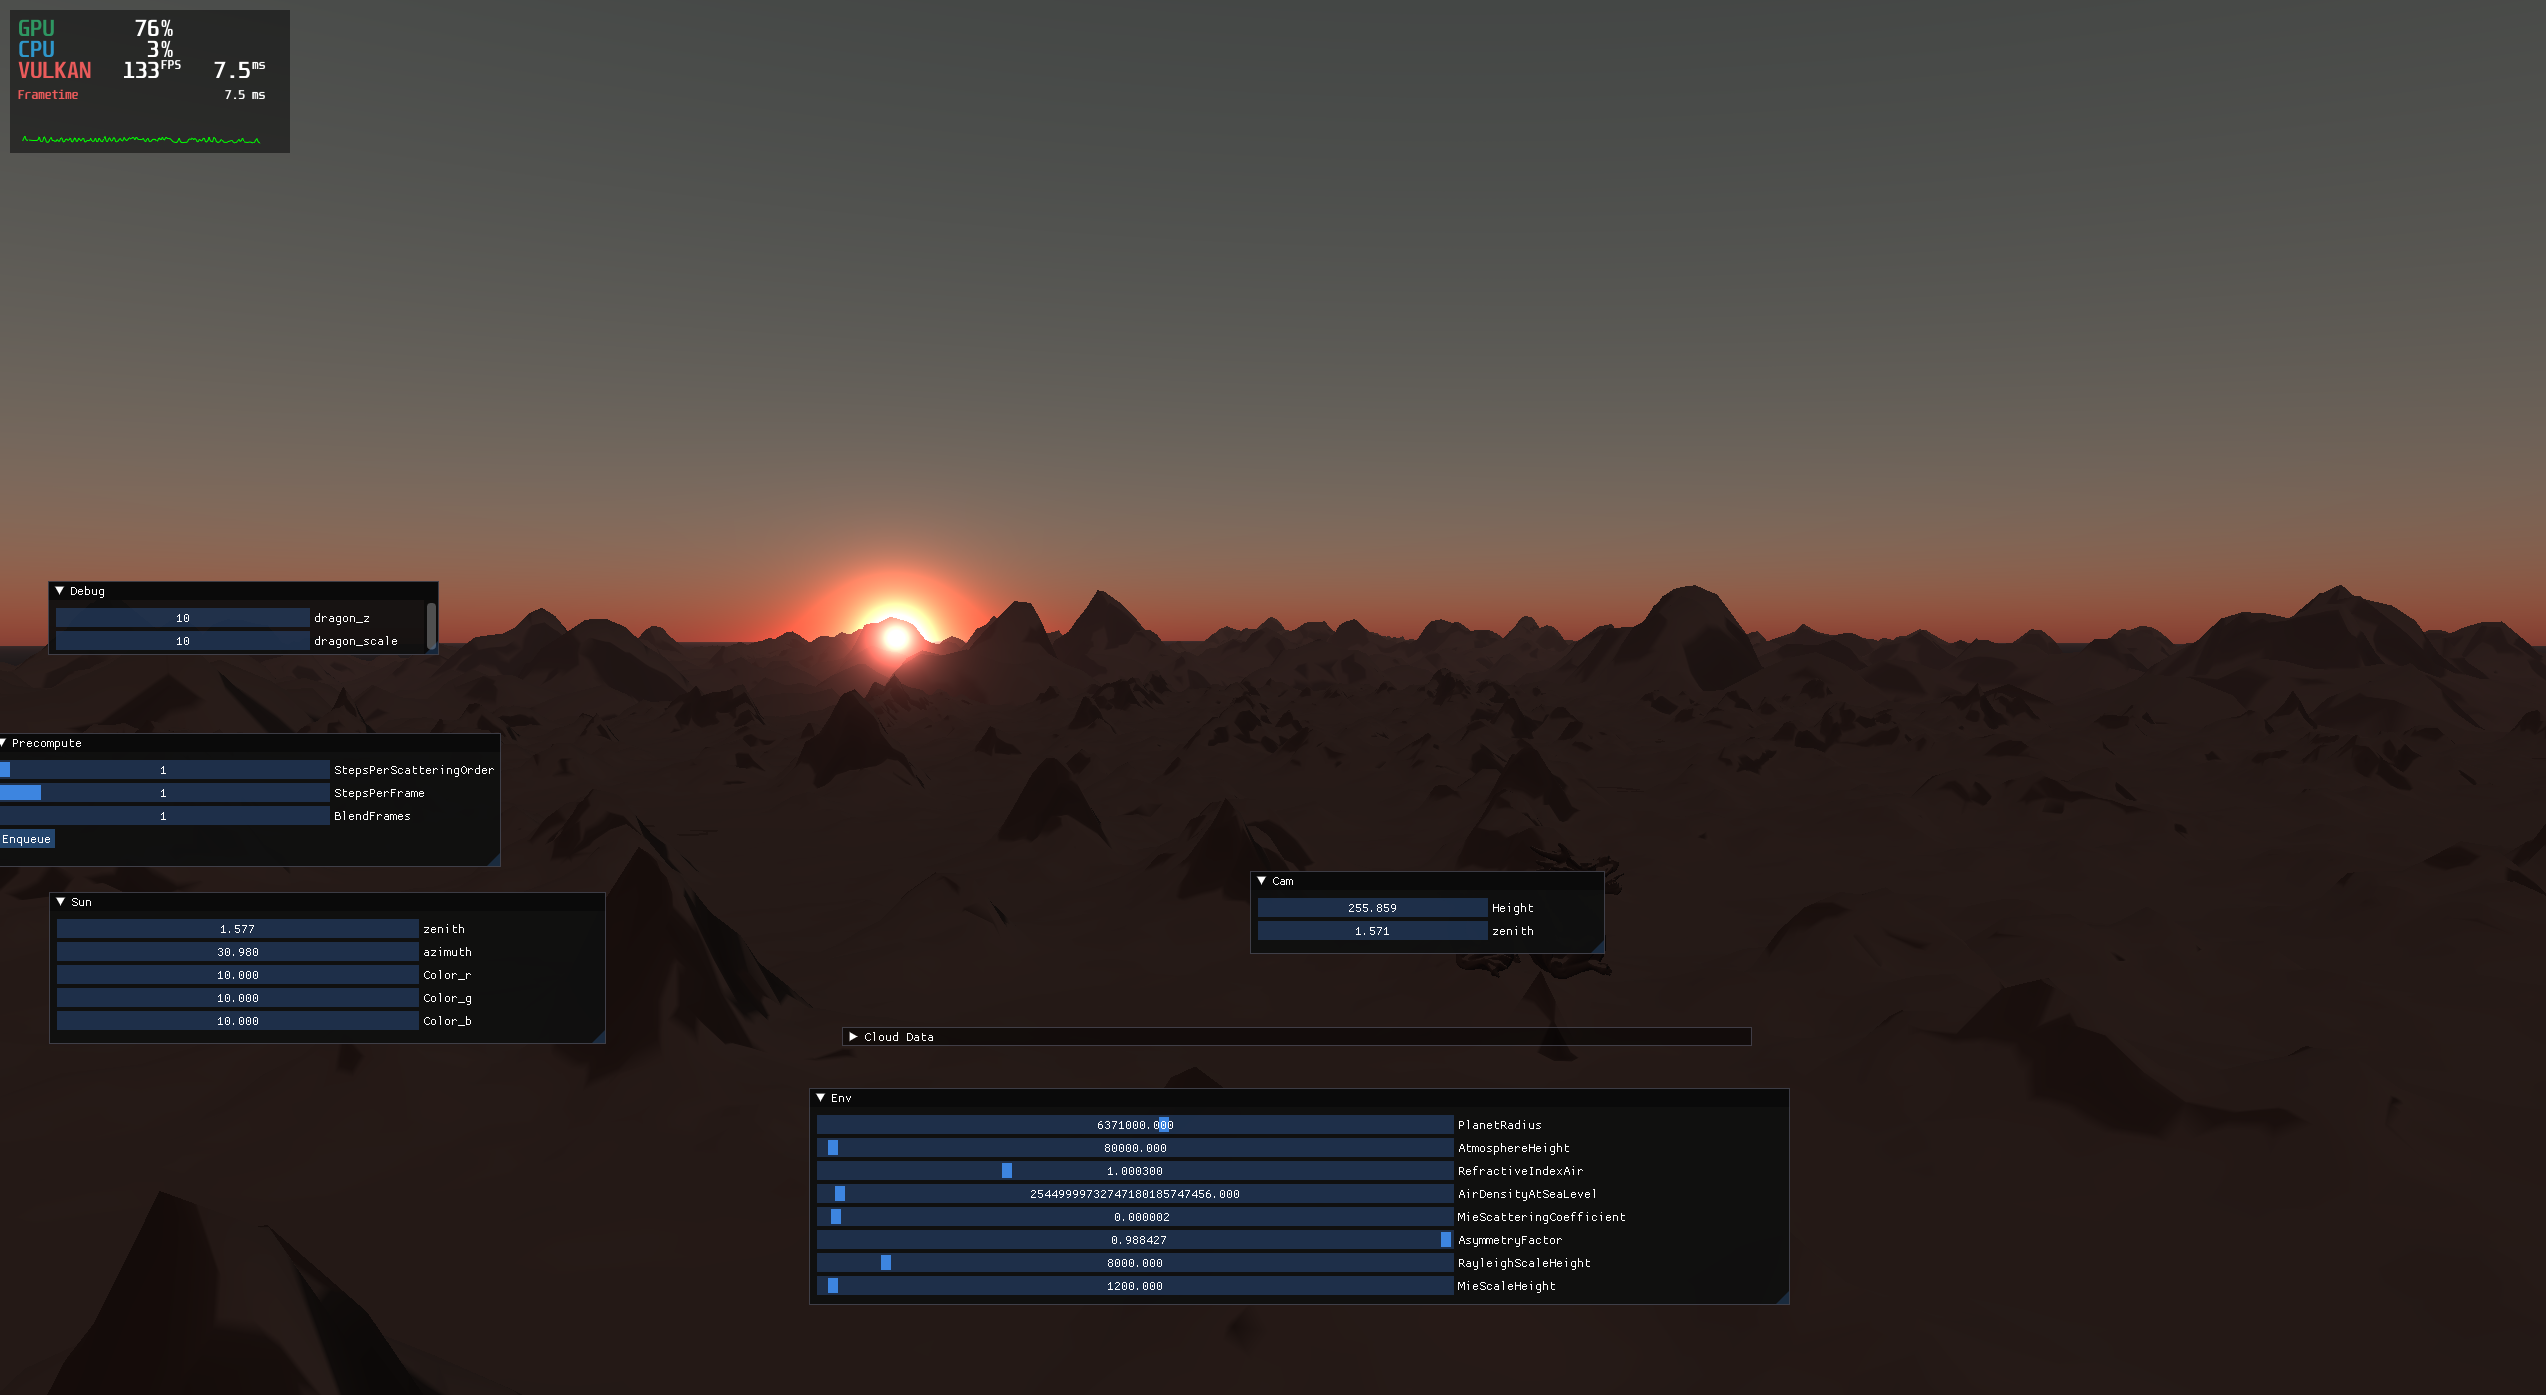
\includegraphics[scale=0.08]{aerial_perspective_improv.png}
\caption{Unverhältnismäßig hohe Mie-Streuung bei Aerial Perspective}
\label{ap_fail}
\end{figure}

\begin{figure}
\centering
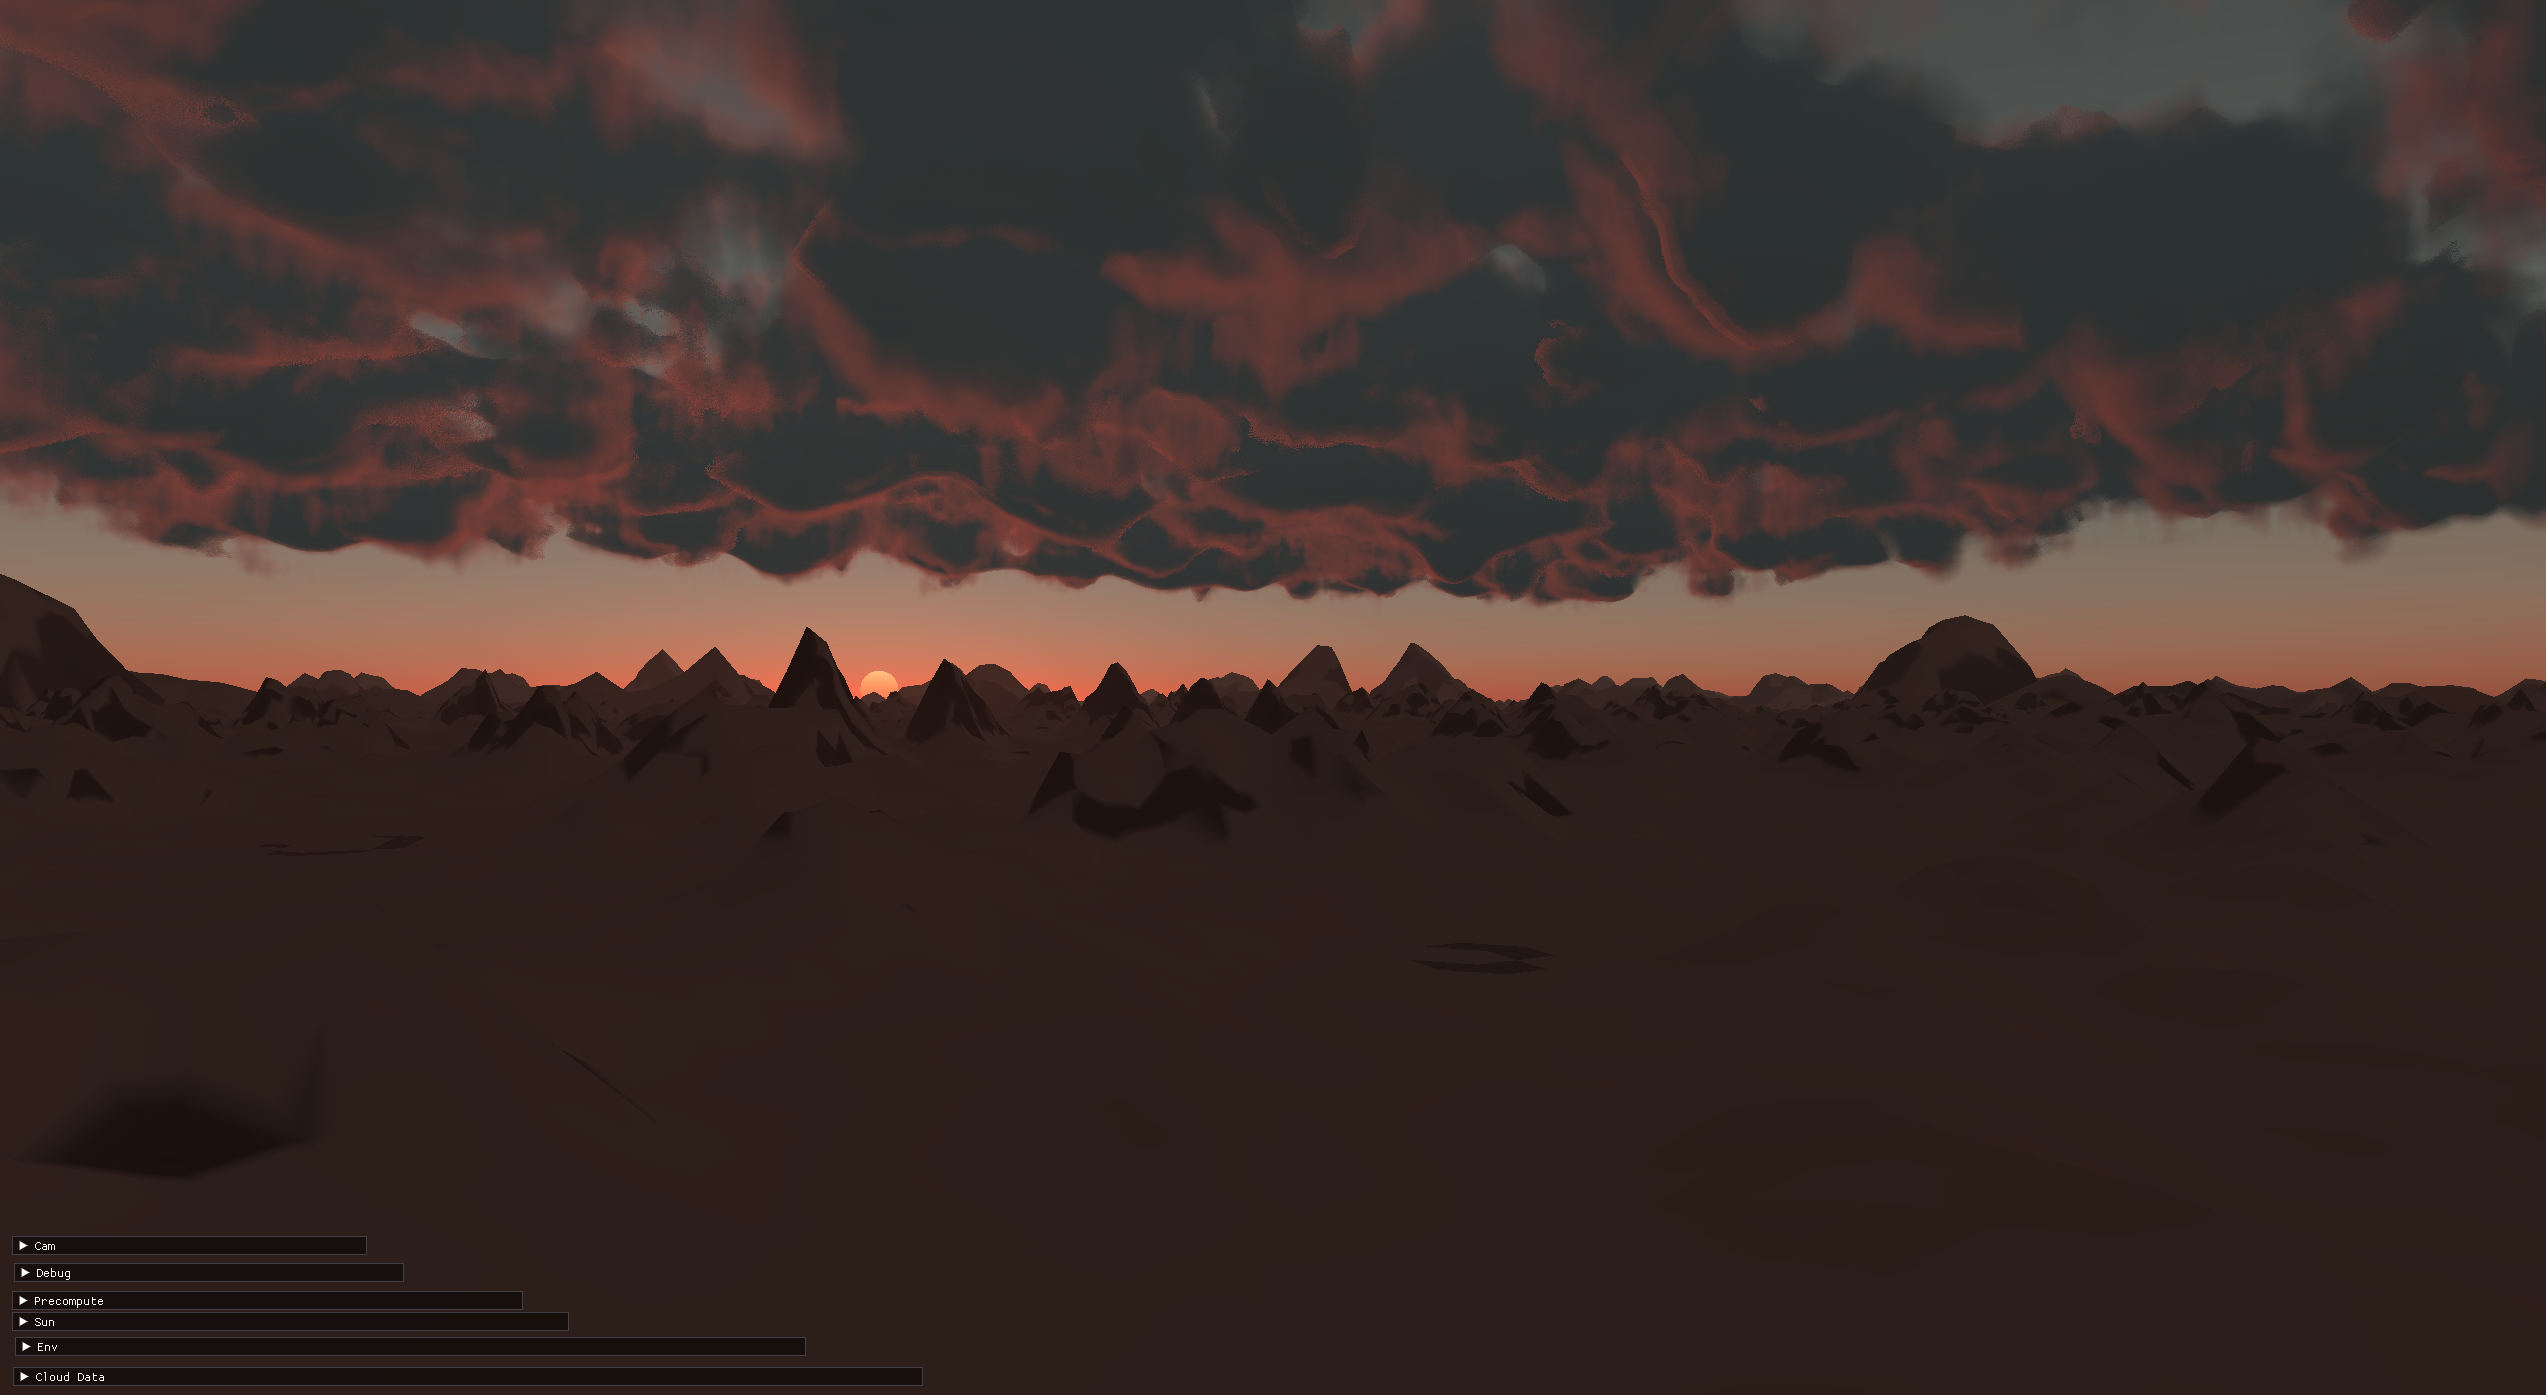
\includegraphics[scale=0.08]{final.png}
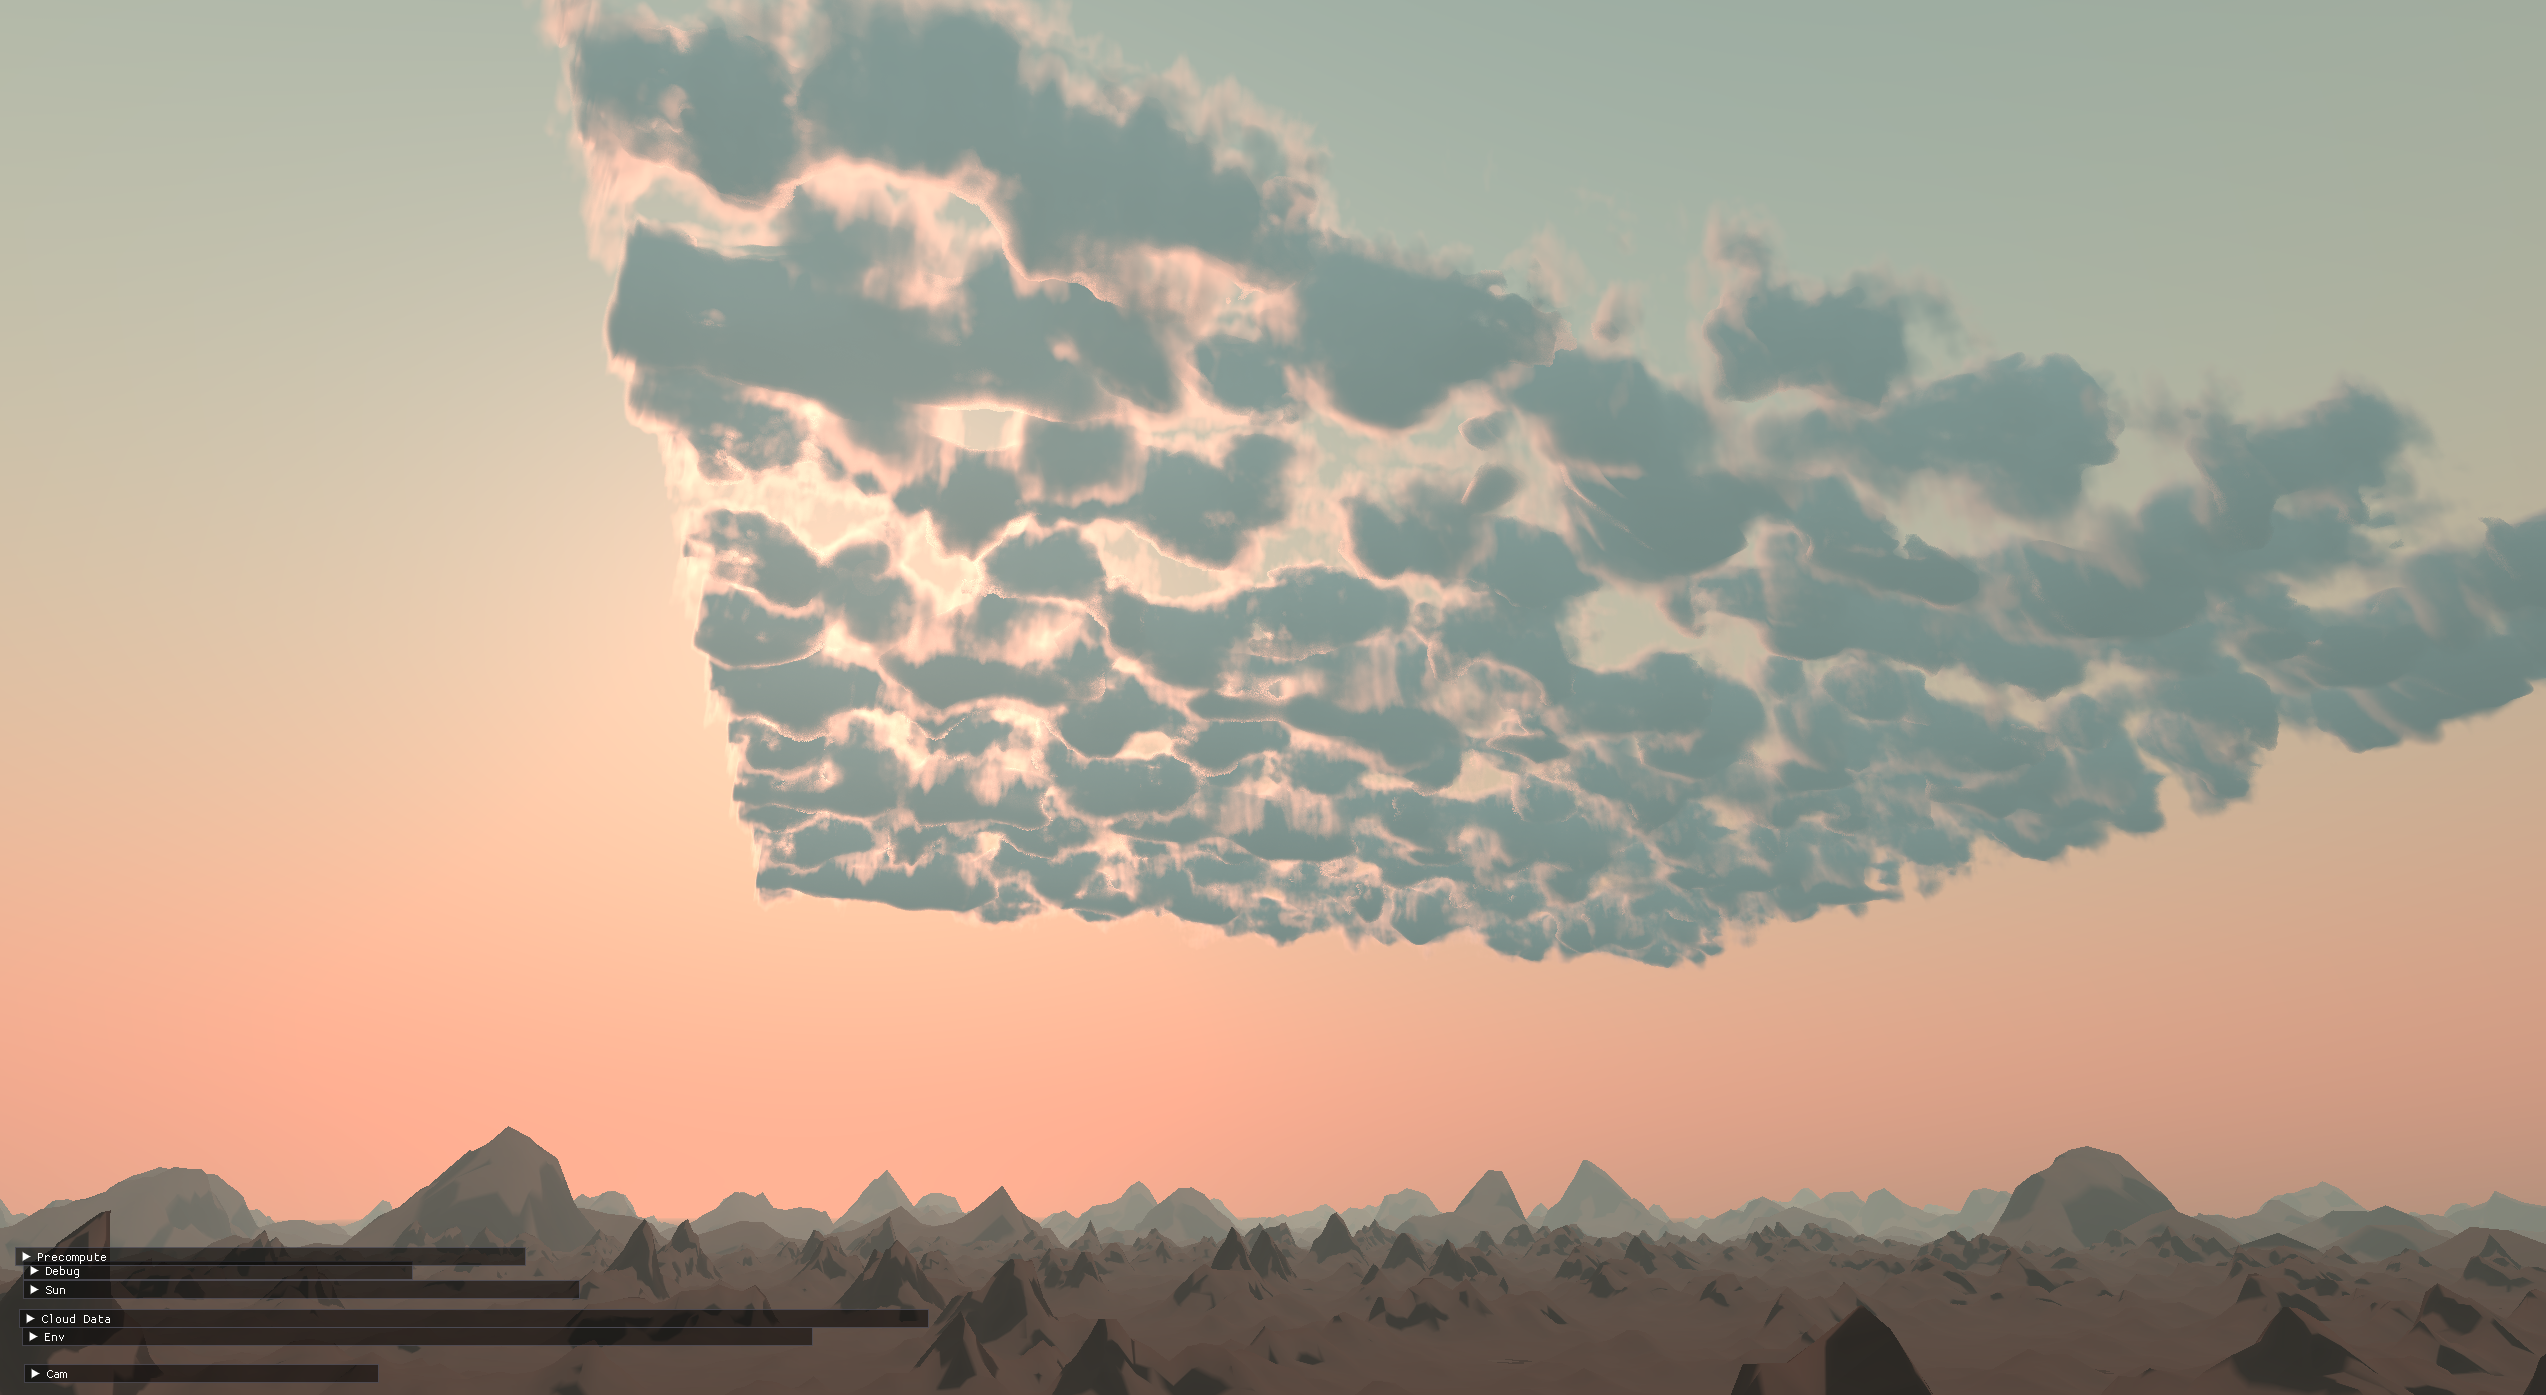
\includegraphics[scale=0.08]{final_high.png}
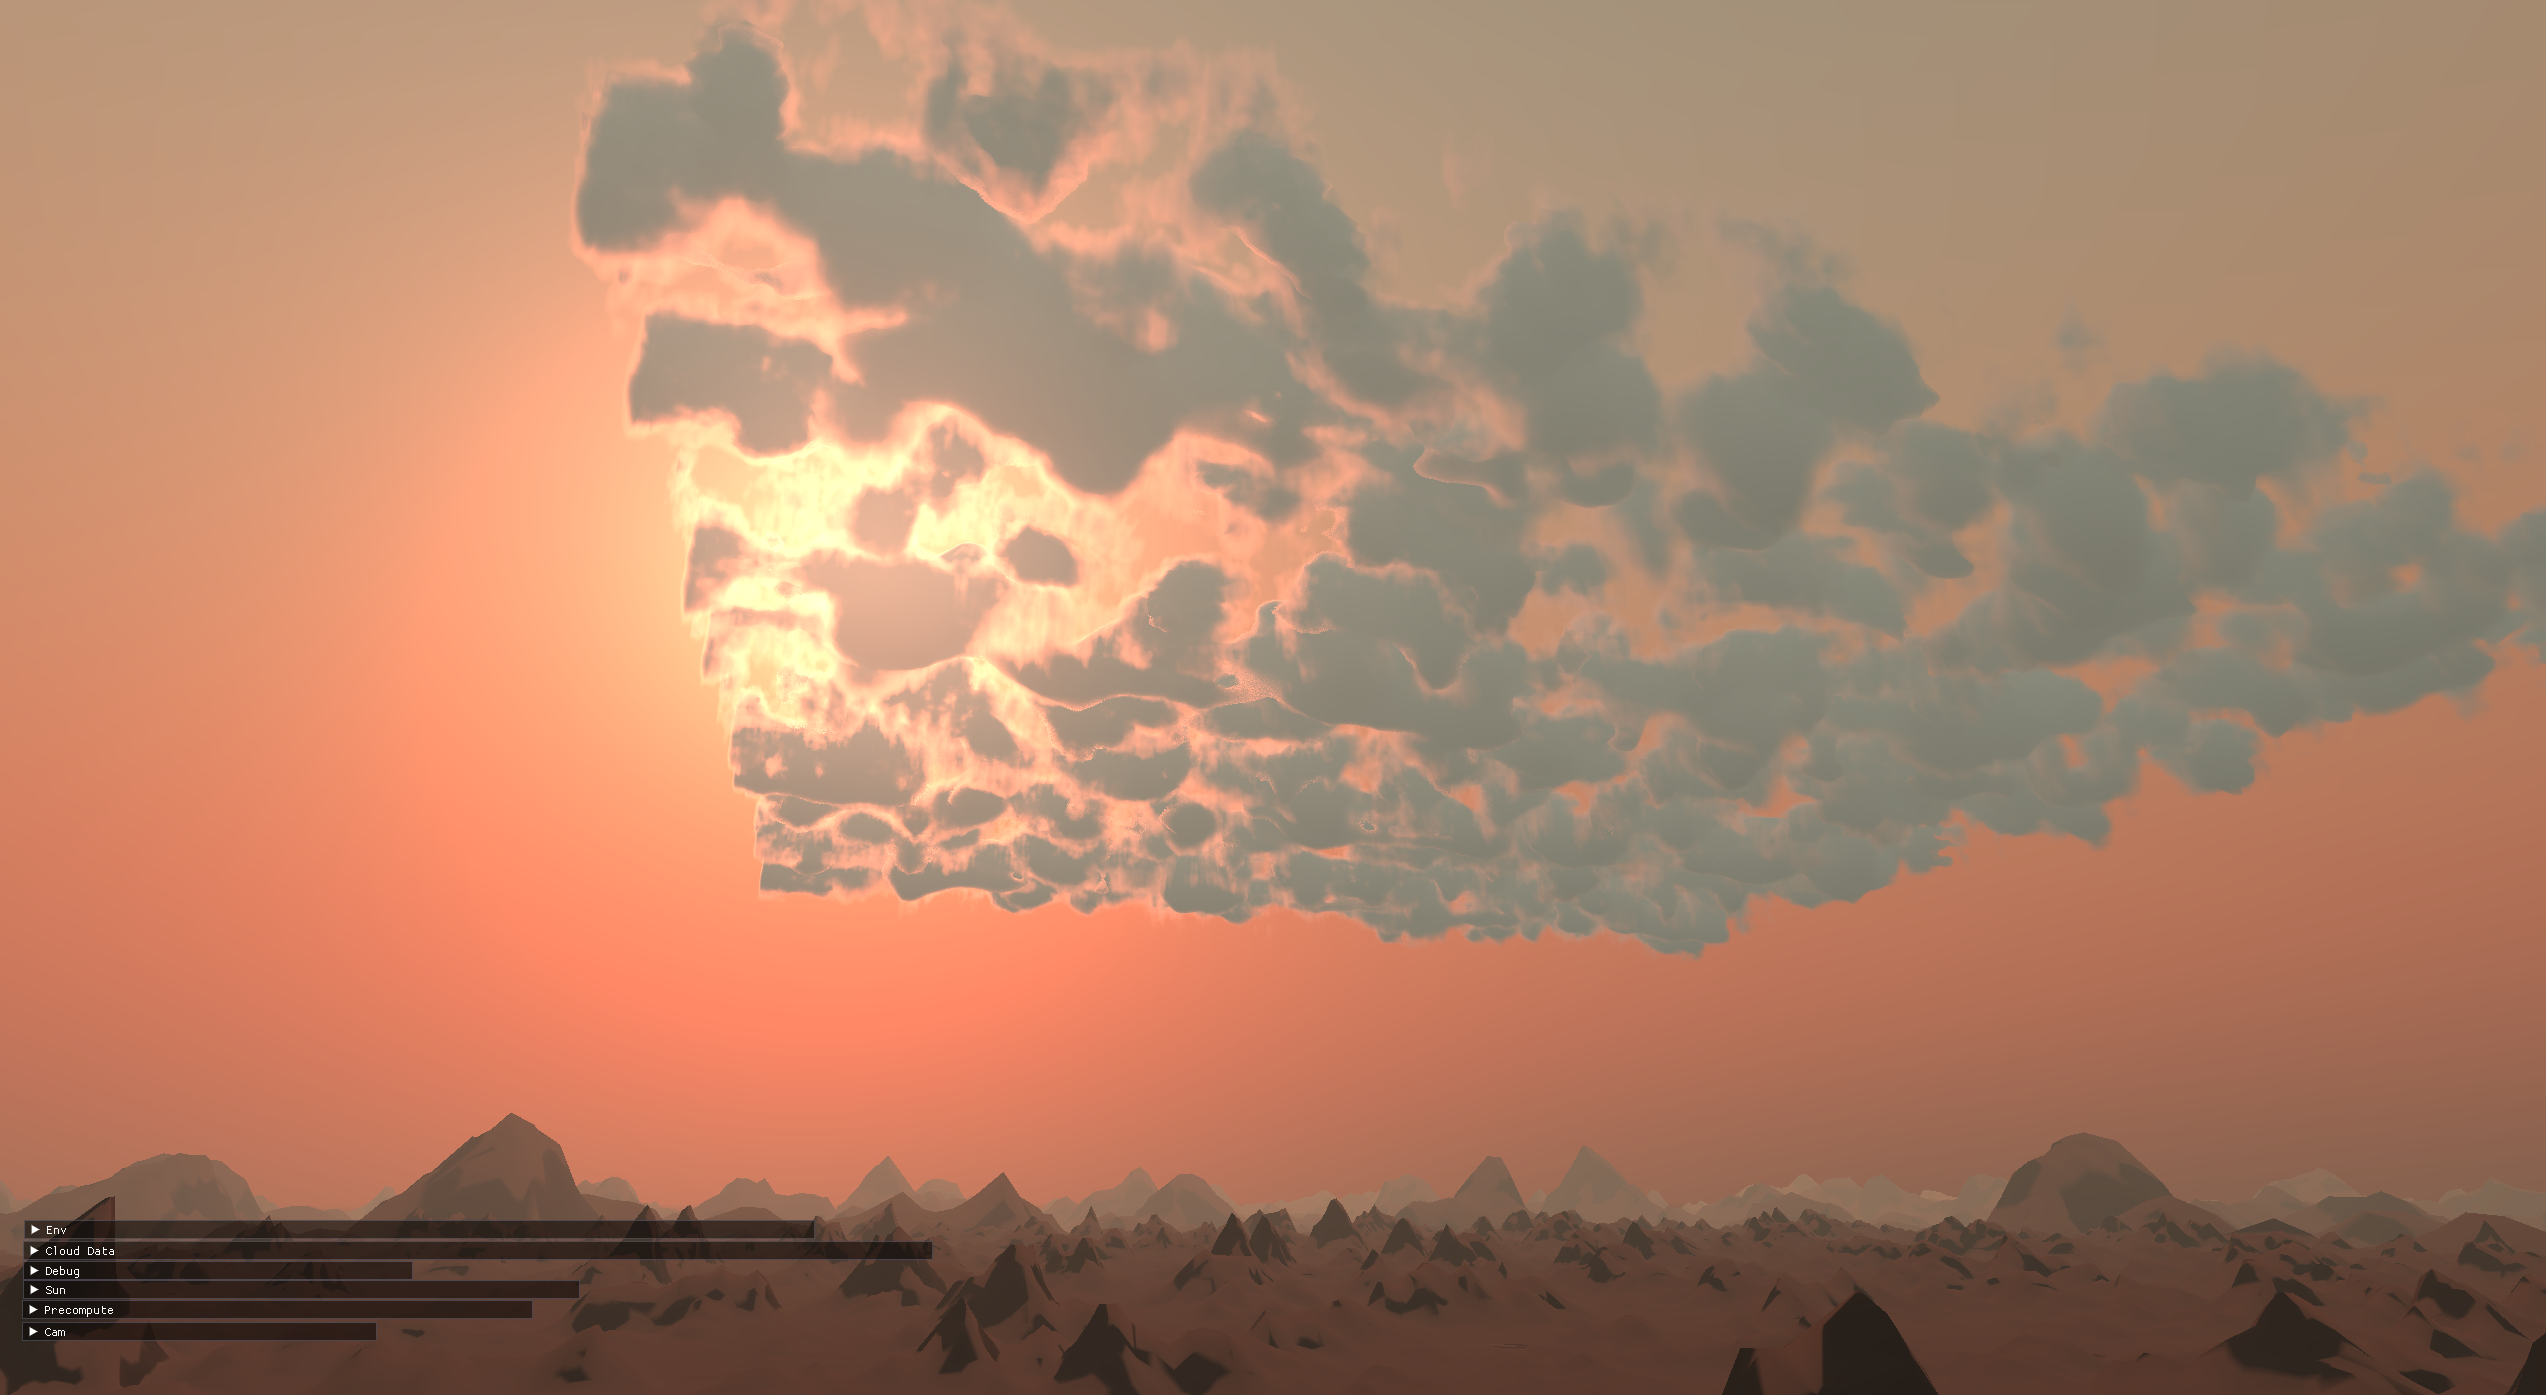
\includegraphics[scale=0.08]{final_high_dens_high_refrIndxAir.png}
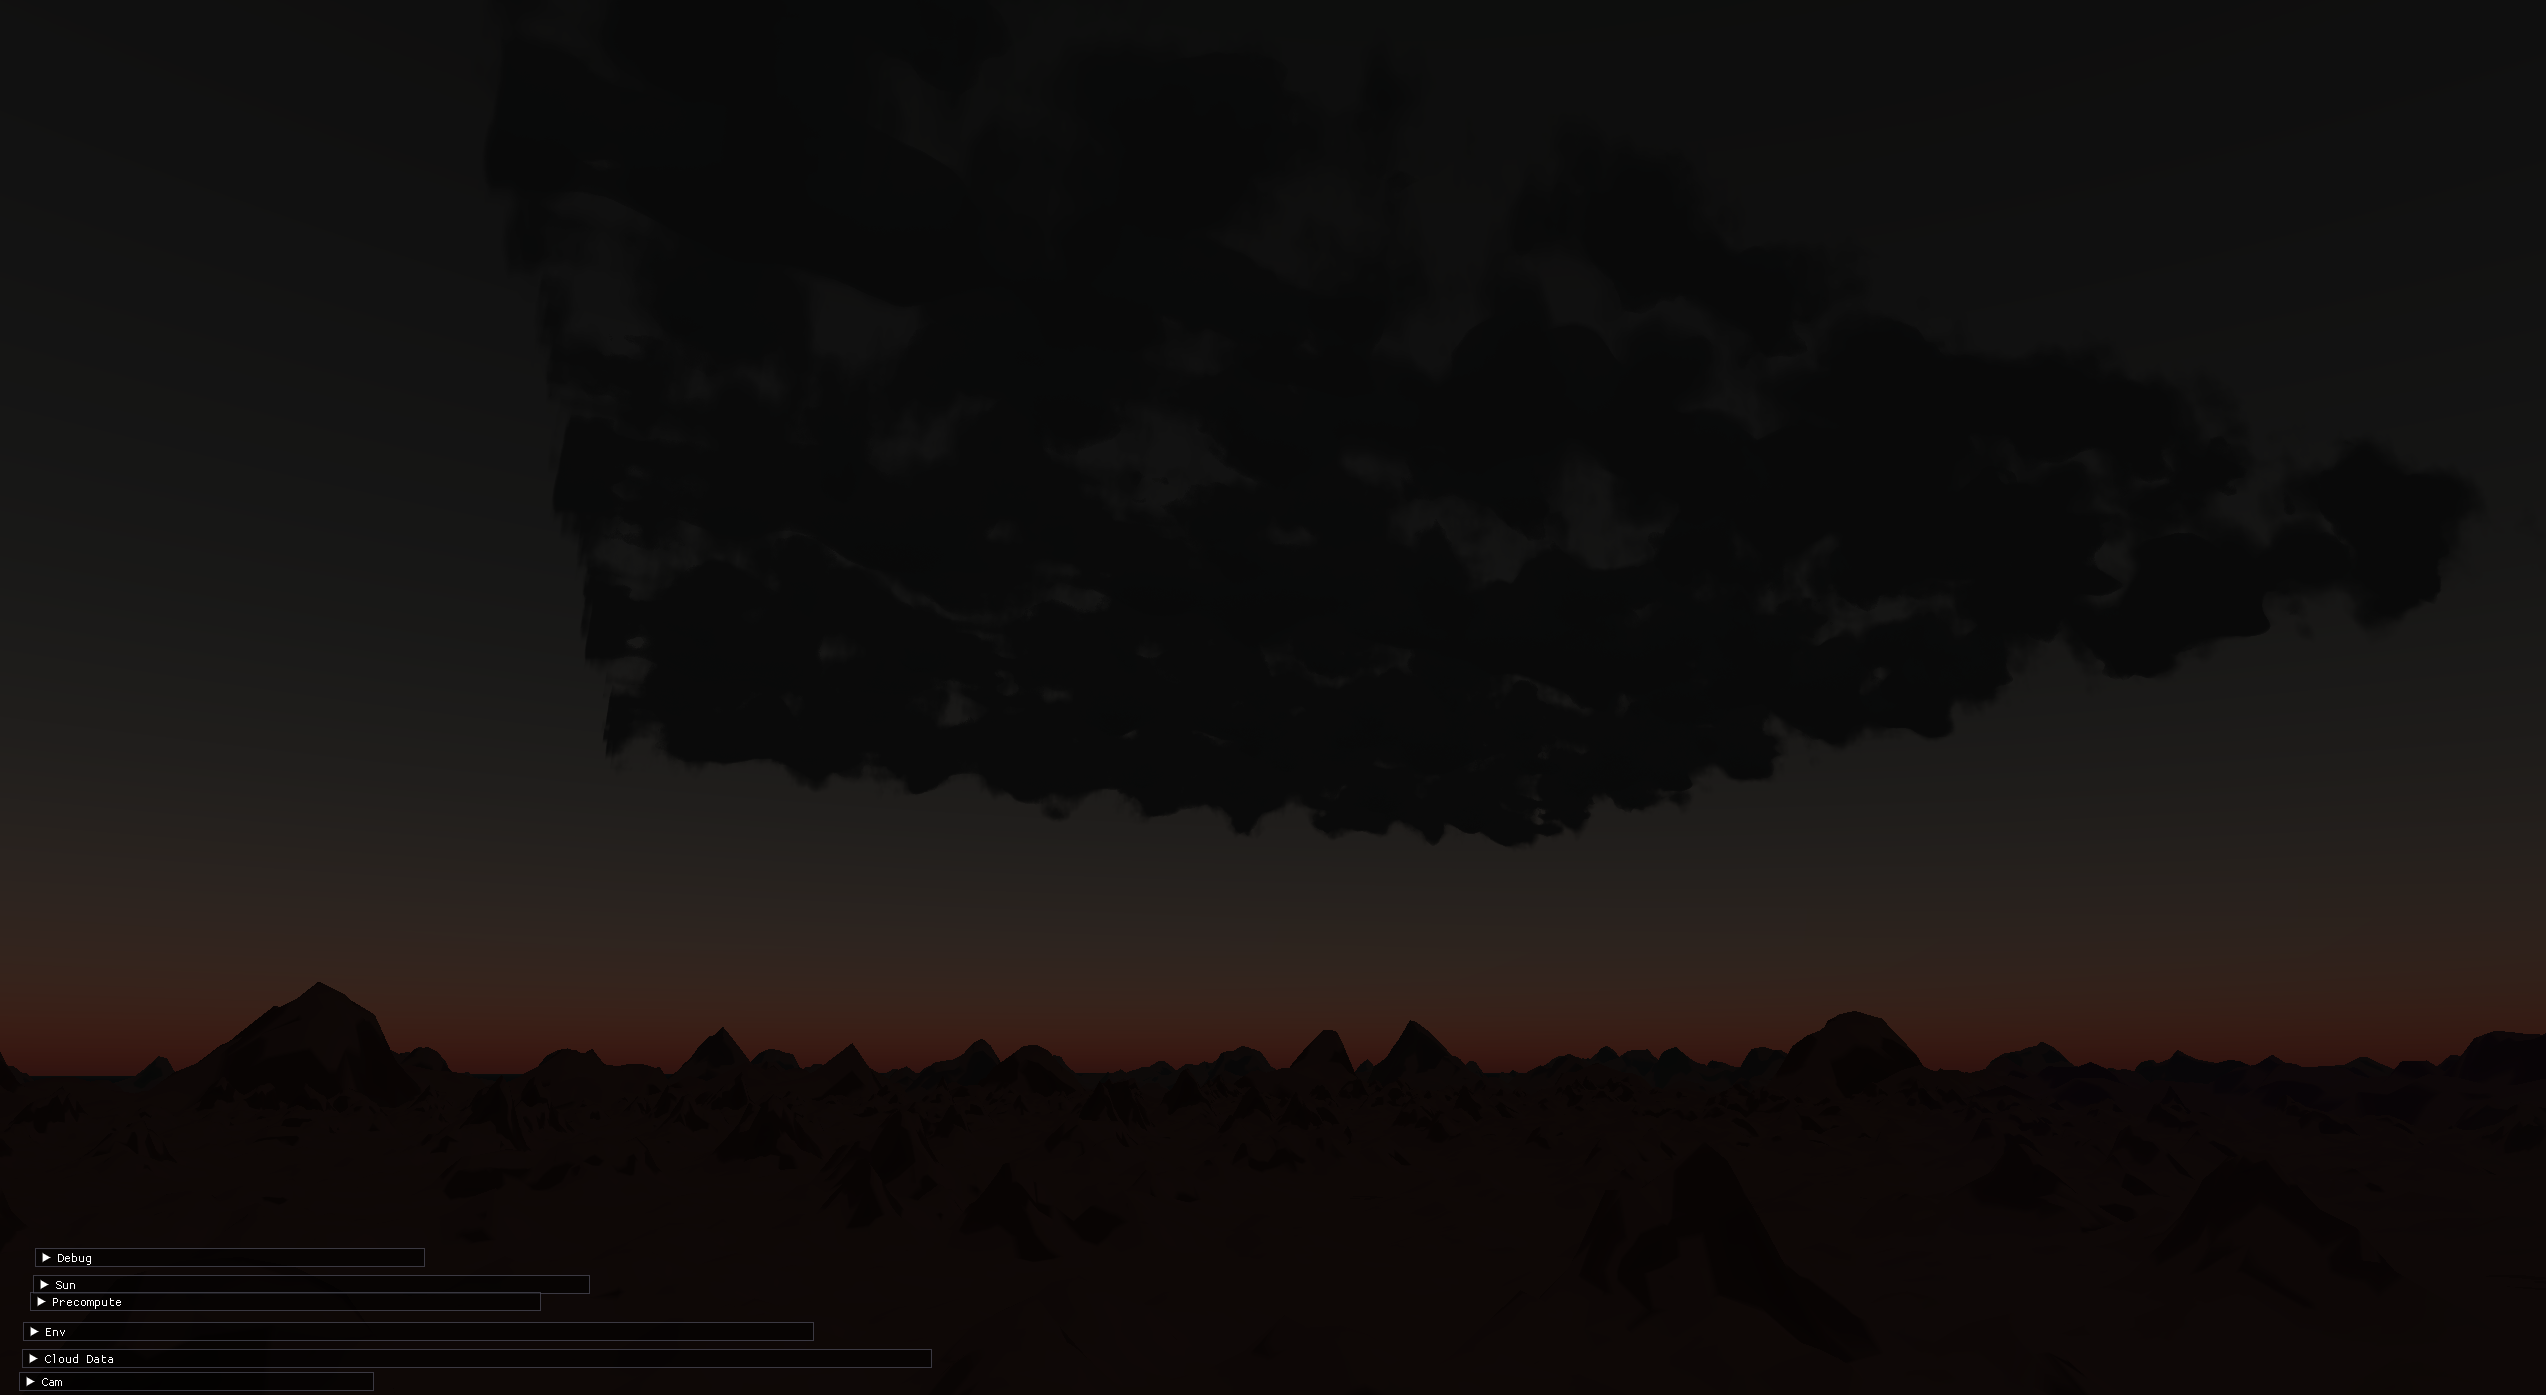
\includegraphics[scale=0.08]{final_twilight.png}
\caption{Der Himmel im kombinierten System (128 primäre und 8 sekundäre Samples bei den Wolken, normale oder hohe Density
für die Atmosphäre)}
\label{final}
\end{figure}
